\chapter{Energy Estimators}
\label{chap:energyestimators}

\chapterquote{There, sir! that is the perfection of vessels!}
{Jules Verne, 1828--1905}

%========================================================================================
%========================================================================================

% Think about splitting this as possible need to redefine these variables....

\section{Novel Energy Estimators}
This section describes two novel energy estimators that are introduced with a view to improving the energy resolution for hadronic showers.  Two techniques will be discussed: HCal hit energy truncation, which focuses on limiting the impact of Landau fluctuations; and software compensation, which focuses on obtaining a compensating calorimeter response.  Both of these techniques are implemented by introducing weights, $\omega^{i}$, to calorimetric energy deposits made by showering particles in the HCal
%
\begin{equation}
E_{Cluster} & = \sum_{ECal \text{ } hits \text{, }i} E^{i}_{ECal} +\sum_{HCal \text{ } hits \text{, }i} E^{i}_{HCal} \omega^{i}(\rho^{i}) \text{ ,}
\label{equ:compensation}
\end{equation}
%
\noindent Weights are only applied to calorimeter hits in the HCal as these techniques modify the energy of hadronic showers, which are primarily contained within the HCal.  The weights, $\omega^{i}$, vary a function of the energy density of the calorimeter hit, $\rho^{i} = E^{i}_{HCal}/V$ where $V$ is the physical volume of a calorimeter hit in the HCal, which includes the both the active and absorber layer thicknesses.  

Although the exact weights depend on the implementation of the technique, a general feature is that at large $E^{i}_{HCal}$ the weight is less than one.  This limits the impact of spuriously high energy hits caused by Landau fluctuations.  The energy loss probability distribution function for scintillator detectors, such as the ILD HCal, is given by a Landau function, which is essentially a Gaussian function with a high energy tail \cite{Landau:1944if}.  Energy deposits from the high energy tail of this distribution, which are known as Landau fluctuations, account for high energy knock-on electrons that appear within particle showers \cite{Bichsel:2004ej}.  As Landau fluctuations deposit a disproportionately large amount of energy with respect to the bulk of the particle shower, they can lead to overestimates of the particle shower energy.  

The energy loss probability distribution function for $n$ particles passing through a calorimeter hit is given by the convolution of $n$ Landau functions, which by the central limits theorem will tend to a Gaussian as $n$ becomes large.  Consequently, as the average number of particles passing through a calorimeter hit increases, the high energy tail in the energy loss probability distribution function for the hit becomes less pronounced and the impact of Landau fluctuations decreases.  This means that the impact of Landau fluctuations on energy measurements is dictated by the density of a particles within a particle shower and the transverse segmentation, or cell size, of the calorimeter in use.  If the transverse segmentation, or cell size, of a calorimeter decreases, the average number of particles passing through each hit decreases and the impact of Landau fluctuations increases.  Any technique used for minimising the impact of Landau fluctuations will be sensitive to the transverse segmentation of the calorimeters in use.  

%========================================================================================

\subsection{HCal Hit Energy Truncation}
\label{sec:hcalcelltruncation}
The first technique to be examined is a simple truncation of the hadronic energy, $E$, recorded in any given HCal hit
%
\begin{equation}
E \rightarrow E' =
\begin{cases}
E & \text{if } E < \kappa \text{ ,} \\
\kappa & \text{otherwise} \text{ ,}
\end{cases}
\end{equation}
%
\noindent where $\kappa$ is the value of the truncation.  This improves the energy estimators for hadronic clusters by limiting the impact of Landau fluctuations.  In terms of $\omega$ introduced in equation \ref{equ:compensation} the truncation corresponds to
%
\begin{equation}
\omega(\rho) =
\begin{cases}
1 & \text{if } \rho \times V < \kappa \text{ ,} \\
\frac{\kappa}{\rho \times V} & \text{otherwise} \text{ .}
\end{cases}
\end{equation}
%
\noindent This weight as a function of hit energy density is shown in figure \ref{fig:hcalcellweight}.  

\begin{figure}[h!]
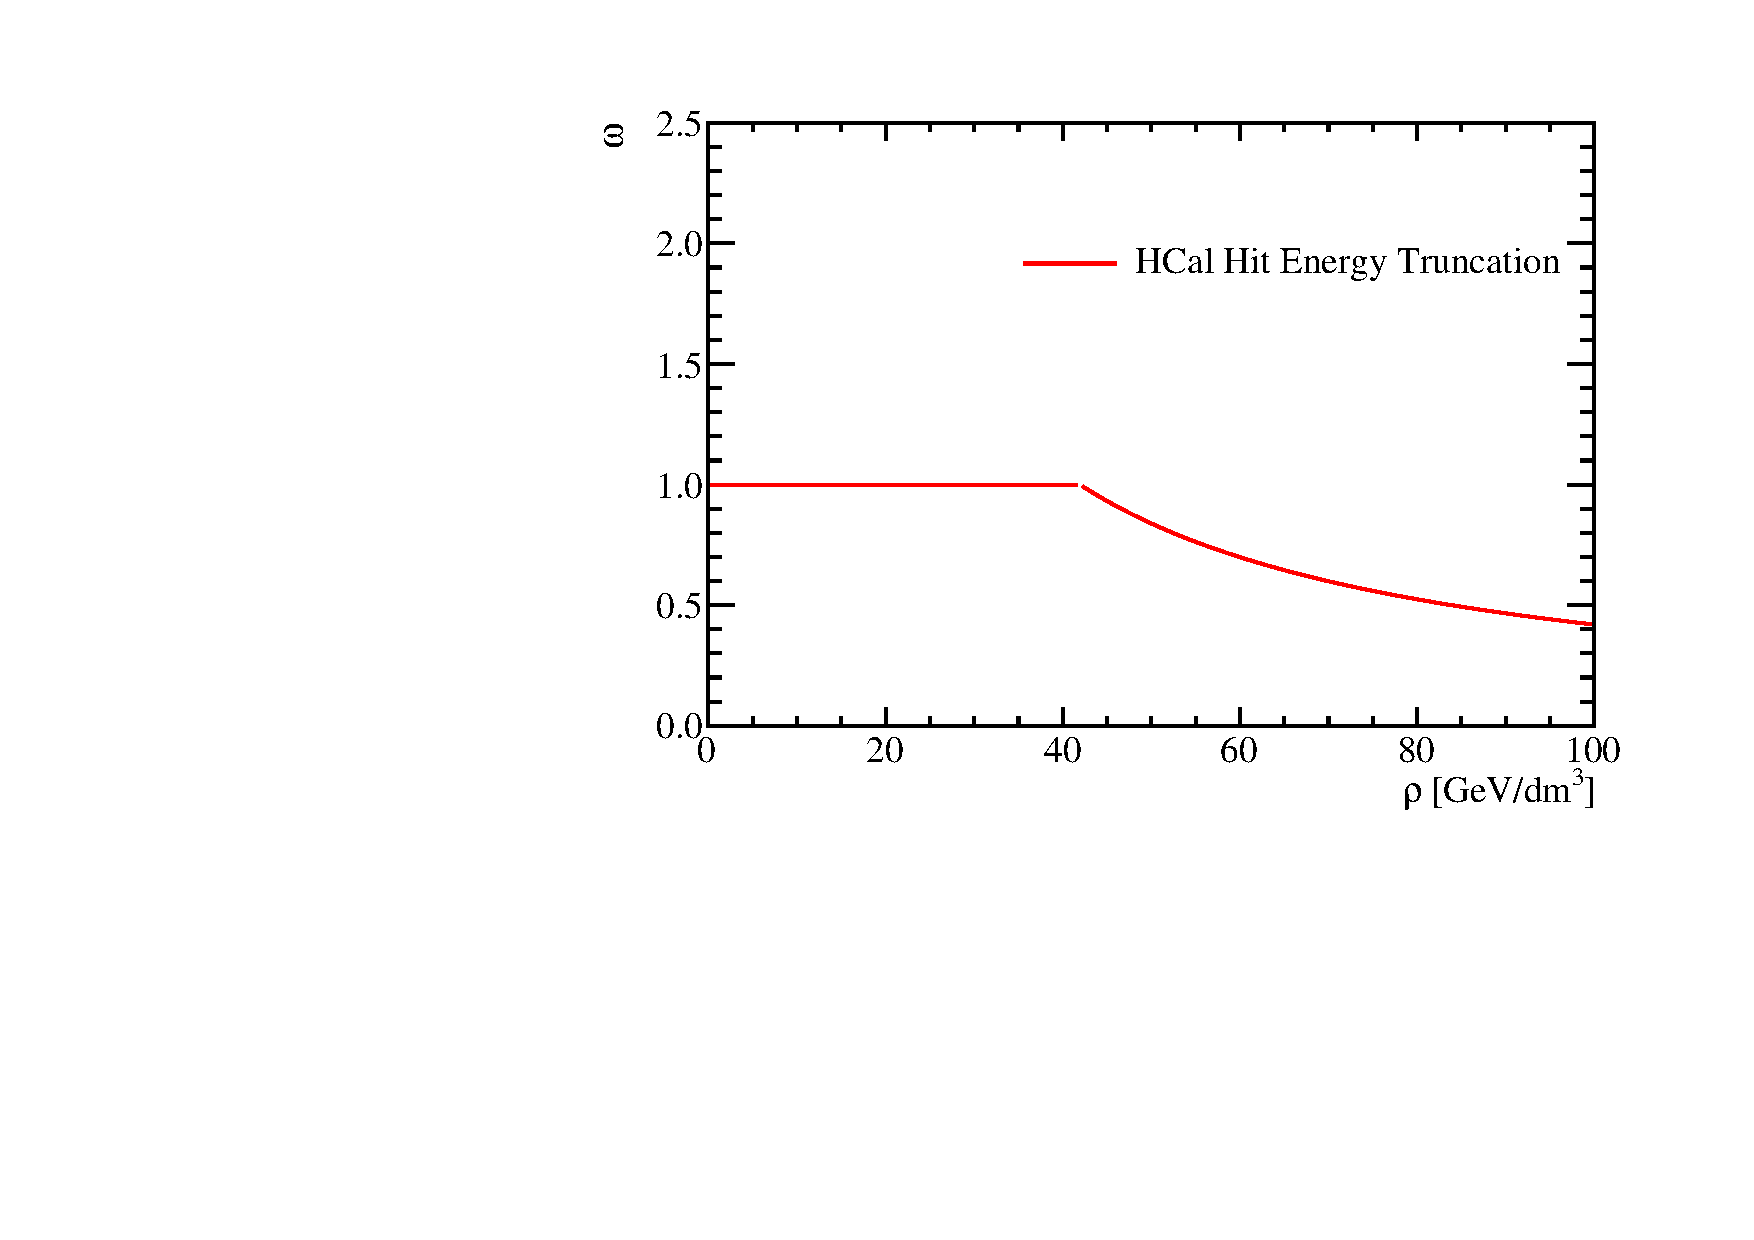
\includegraphics[width=0.5\textwidth]{EnergyEstimators/Plots/SoftComp/Weights/CellTruncWeights.pdf}
\caption[The weights, $\omega$, used in the HCal hit energy truncation as a function of the energy density of the HCal hit, $\rho$.  The truncation shown here corresponds to a 1~GeV truncation in the nominal ILD HCal.]{The weights, $\omega$, used in the HCal hit energy truncation as a function of the energy density of the HCal hit, $\rho$.  The truncation shown here corresponds to a 1~GeV truncation in the nominal ILD HCal.}
\label{fig:hcalcellweight}
\end{figure}

%========================================================================================

\subsubsection{Impact on Single Particle Energy Resolution}
Figure \ref{fig:ercelltrunckaons} shows the energy resolution for neutral hadrons as a function of the HCal hit energy truncation.  The optimal truncation for the ILD detector model simulation was 1~GeV and, using this truncation, a neutral hadron energy resolution of $\sim$8.8\% was obtained.  This energy resolution is approximately $\sim$1.6\% lower than that obtained without the use of a truncation.  Smaller energy truncations begin to truncate the energy of calorimeter hits produced in typical hadronic shower development, while larger truncations allow for a larger impact from Landau fluctuations.  Both of these effects result in worsening neutral hadron energy resolutions.  For completeness the $\gamma$ energy resolutions as a function of HCal hit energy truncation are shown in figure \ref{fig:ercelltruncphotons}.  As expected the $\gamma$ energy resolution is unaffected by the HCal hit energy truncation as the $\gamma$s are largely contained within the ECal.

\begin{figure}[h!]
\subfloat[]{\label{fig:ercelltrunckaons}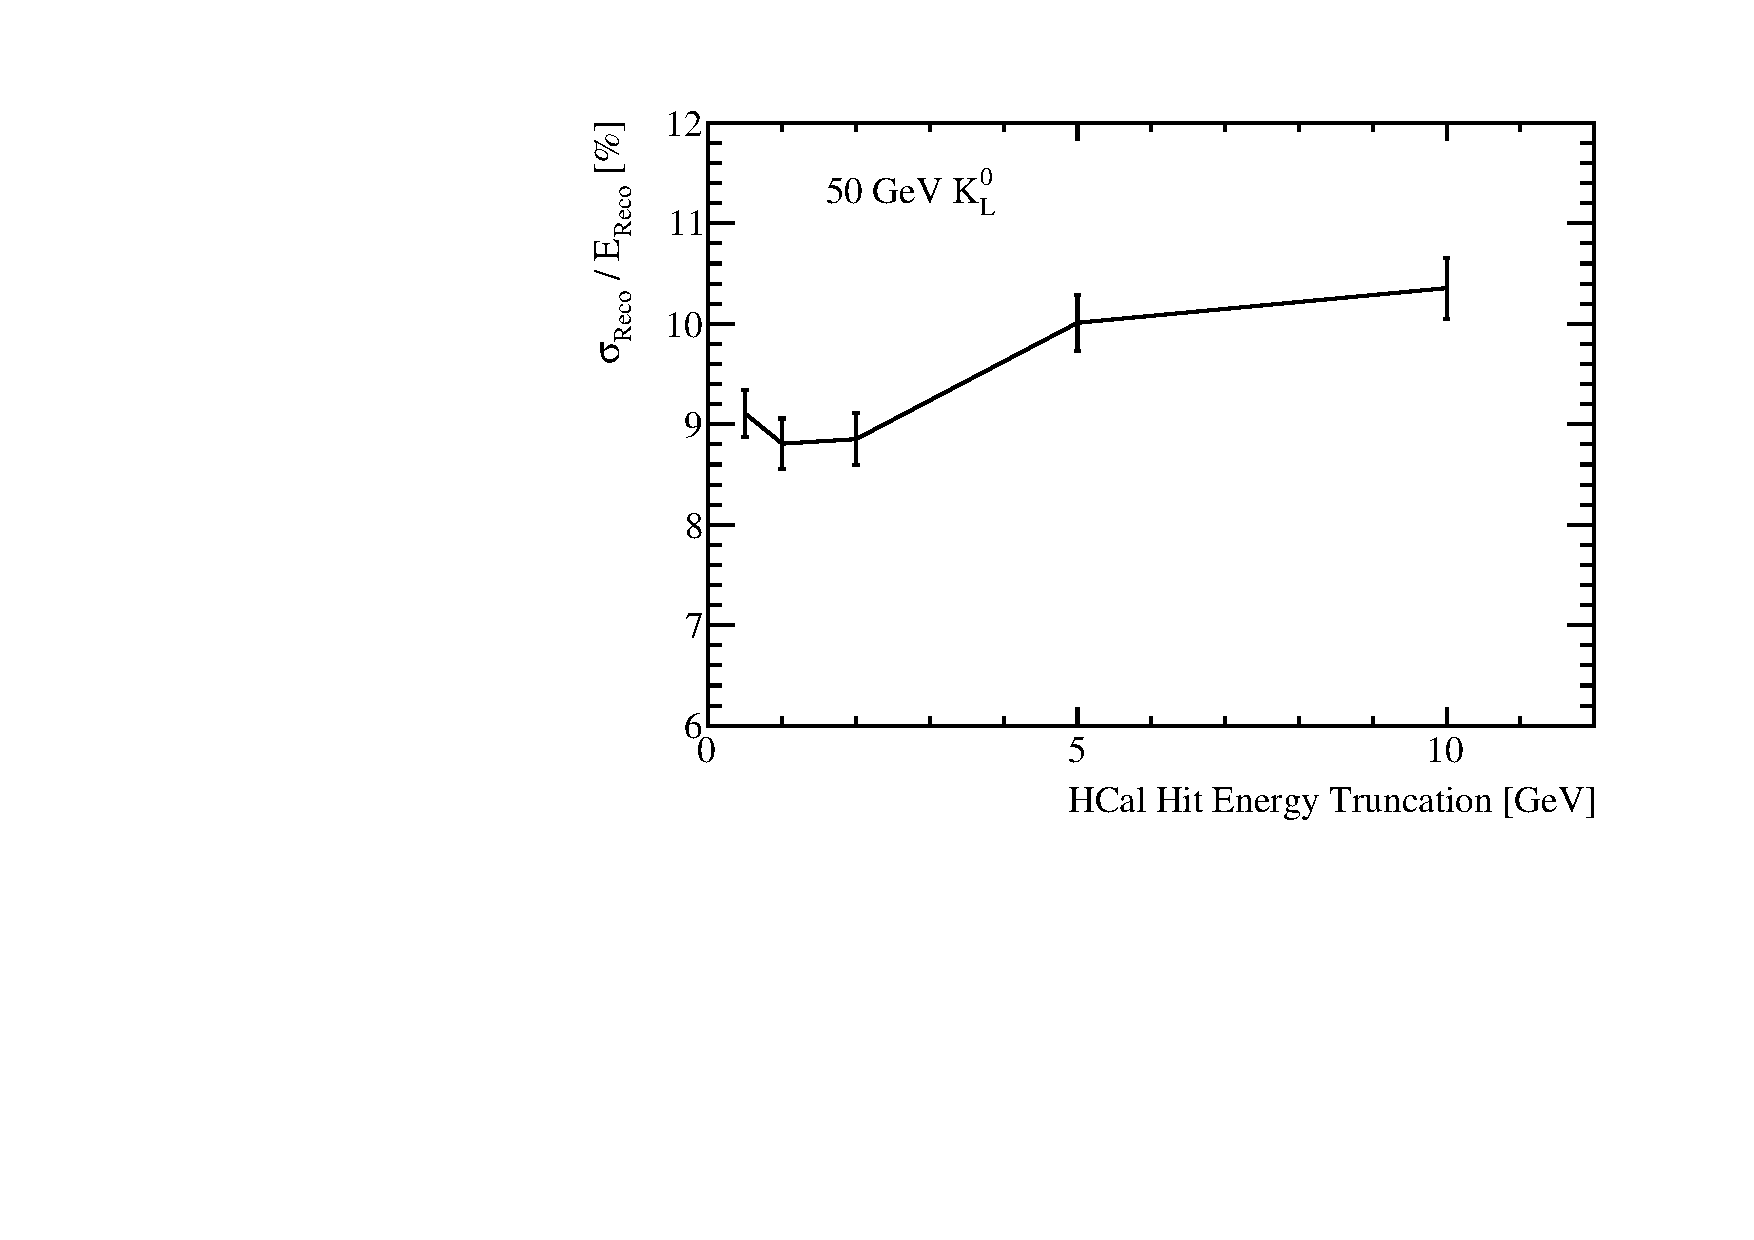
\includegraphics[width=0.5\textwidth]{EnergyEstimators/Plots/CellTruncation/ER_vs_Kaon0LCellTrunc_50GeVKaon0L.pdf}}
\subfloat[]{\label{fig:ercelltruncphotons}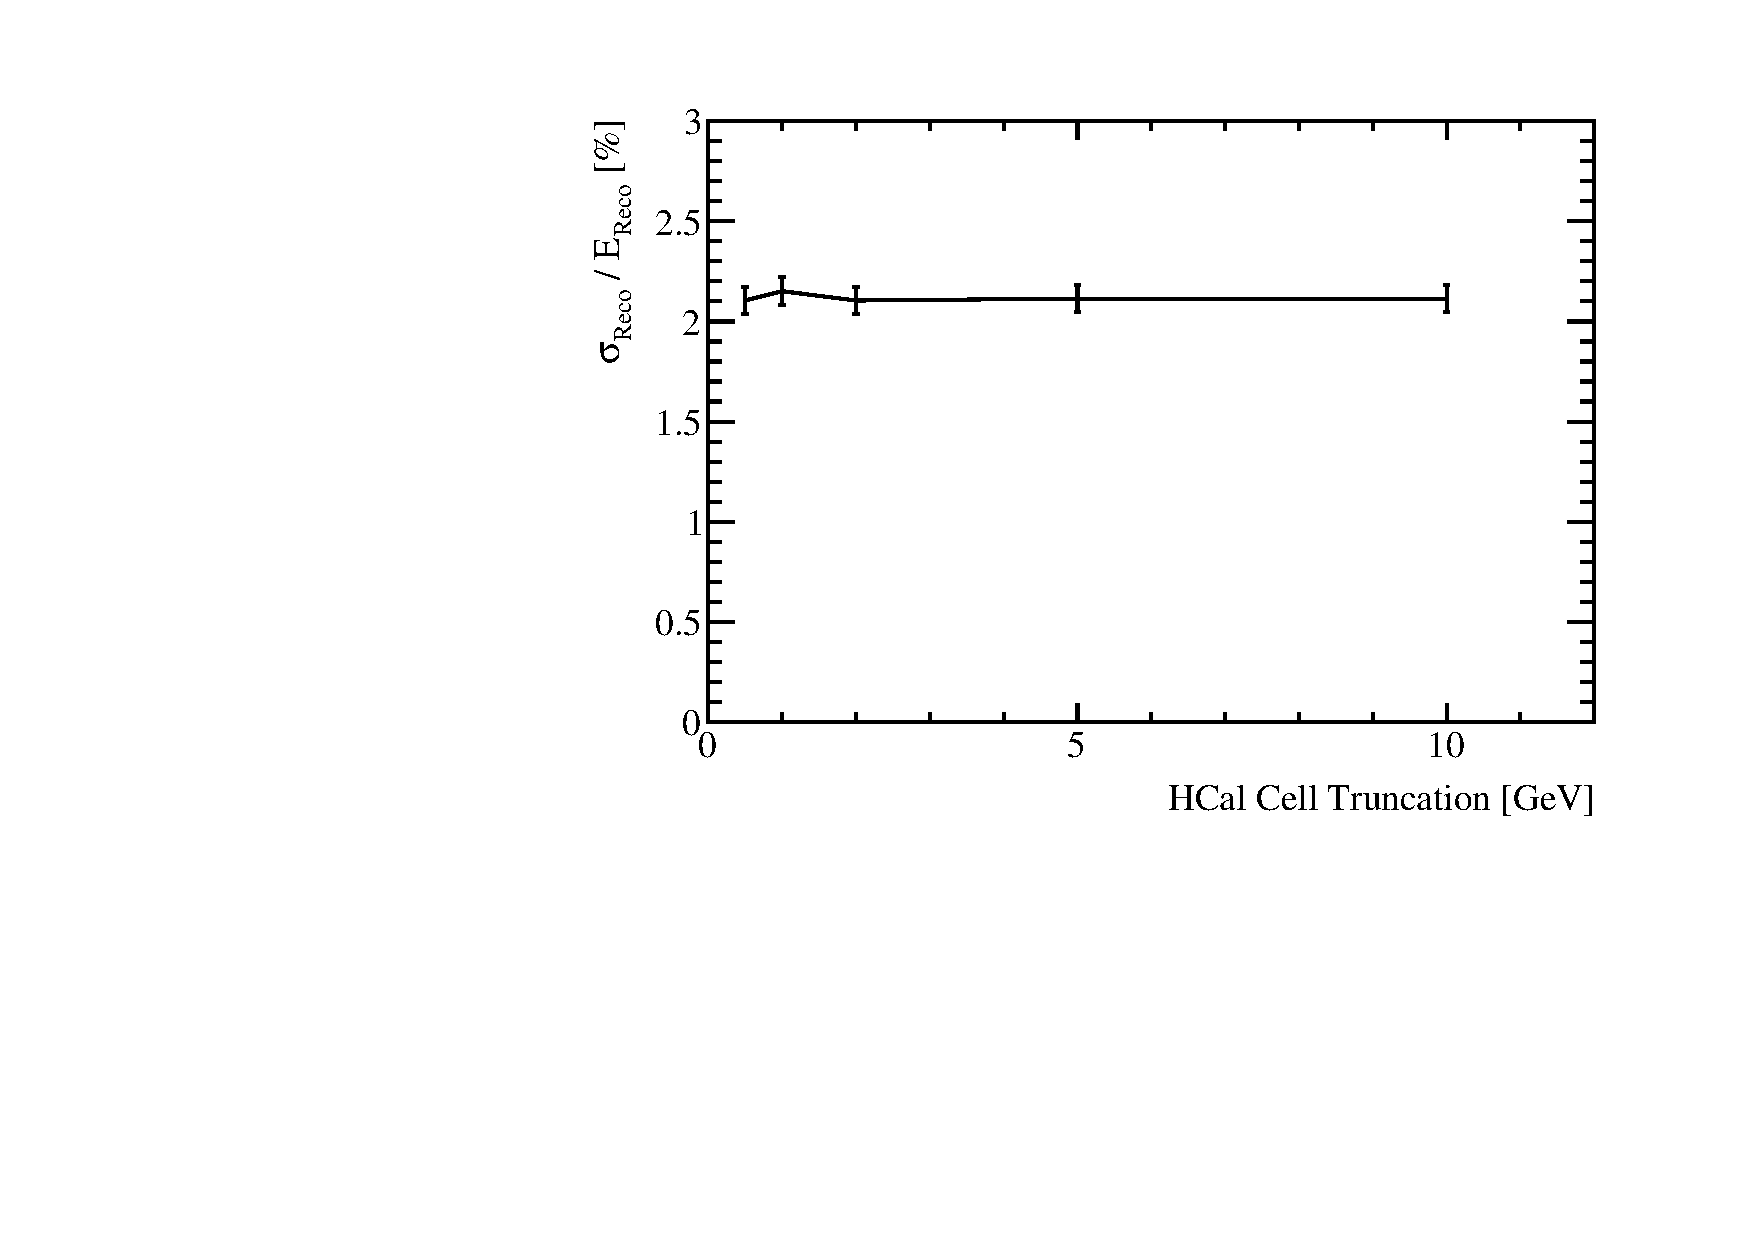
\includegraphics[width=0.5\textwidth]{EnergyEstimators/Plots/CellTruncation/ER_vs_PhotonCellTrunc_100GeVPhoton.pdf}}
\caption[The energy resolution as a function of HCal cell truncation for \protect\subref{fig:ercelltrunckaons} 50~GeV $K^{0}_{L}$ events and \protect\subref{fig:ercelltruncphotons} 100~GeV $\gamma$ events using the nominal ILD detector model.]{The energy resolution as a function of HCal cell truncation for \protect\subref{fig:ercelltrunckaons} 50~GeV $K^{0}_{L}$ events and \protect\subref{fig:ercelltruncphotons} 100~GeV $\gamma$ events using the nominal ILD detector model.}
\label{fig:ercelltrunc}
\end{figure}

%========================================================================================

\subsubsection{Impact on Jet Energy Resolution}
Figure \ref{fig:jercelltrunc} shows the jet energy resolution as a function of jet energy for selected values of the HCal hit energy truncation.  The trends in this plot are complex as the optimal HCal hit energy truncation varies with the jet energy.  For 45.5~GeV jets, the best jet energy resolution, $\sim$3.55\%, is obtained using a 0.5~GeV truncation, while for 180~GeV jets, the best jet energy resolution, $\sim$2.85\%, is obtained using a 1~GeV truncation.  This is expected as at low jet energies the average number of particles passing through each active calorimeter hit will be small, meaning the impact of Landau fluctuations is large and that to limit them a small truncation is needed.  As the jet energy increases more particles on average pass through each calorimeter hit and the impact of Landau fluctuations decreases.  

\begin{figure}[h!]
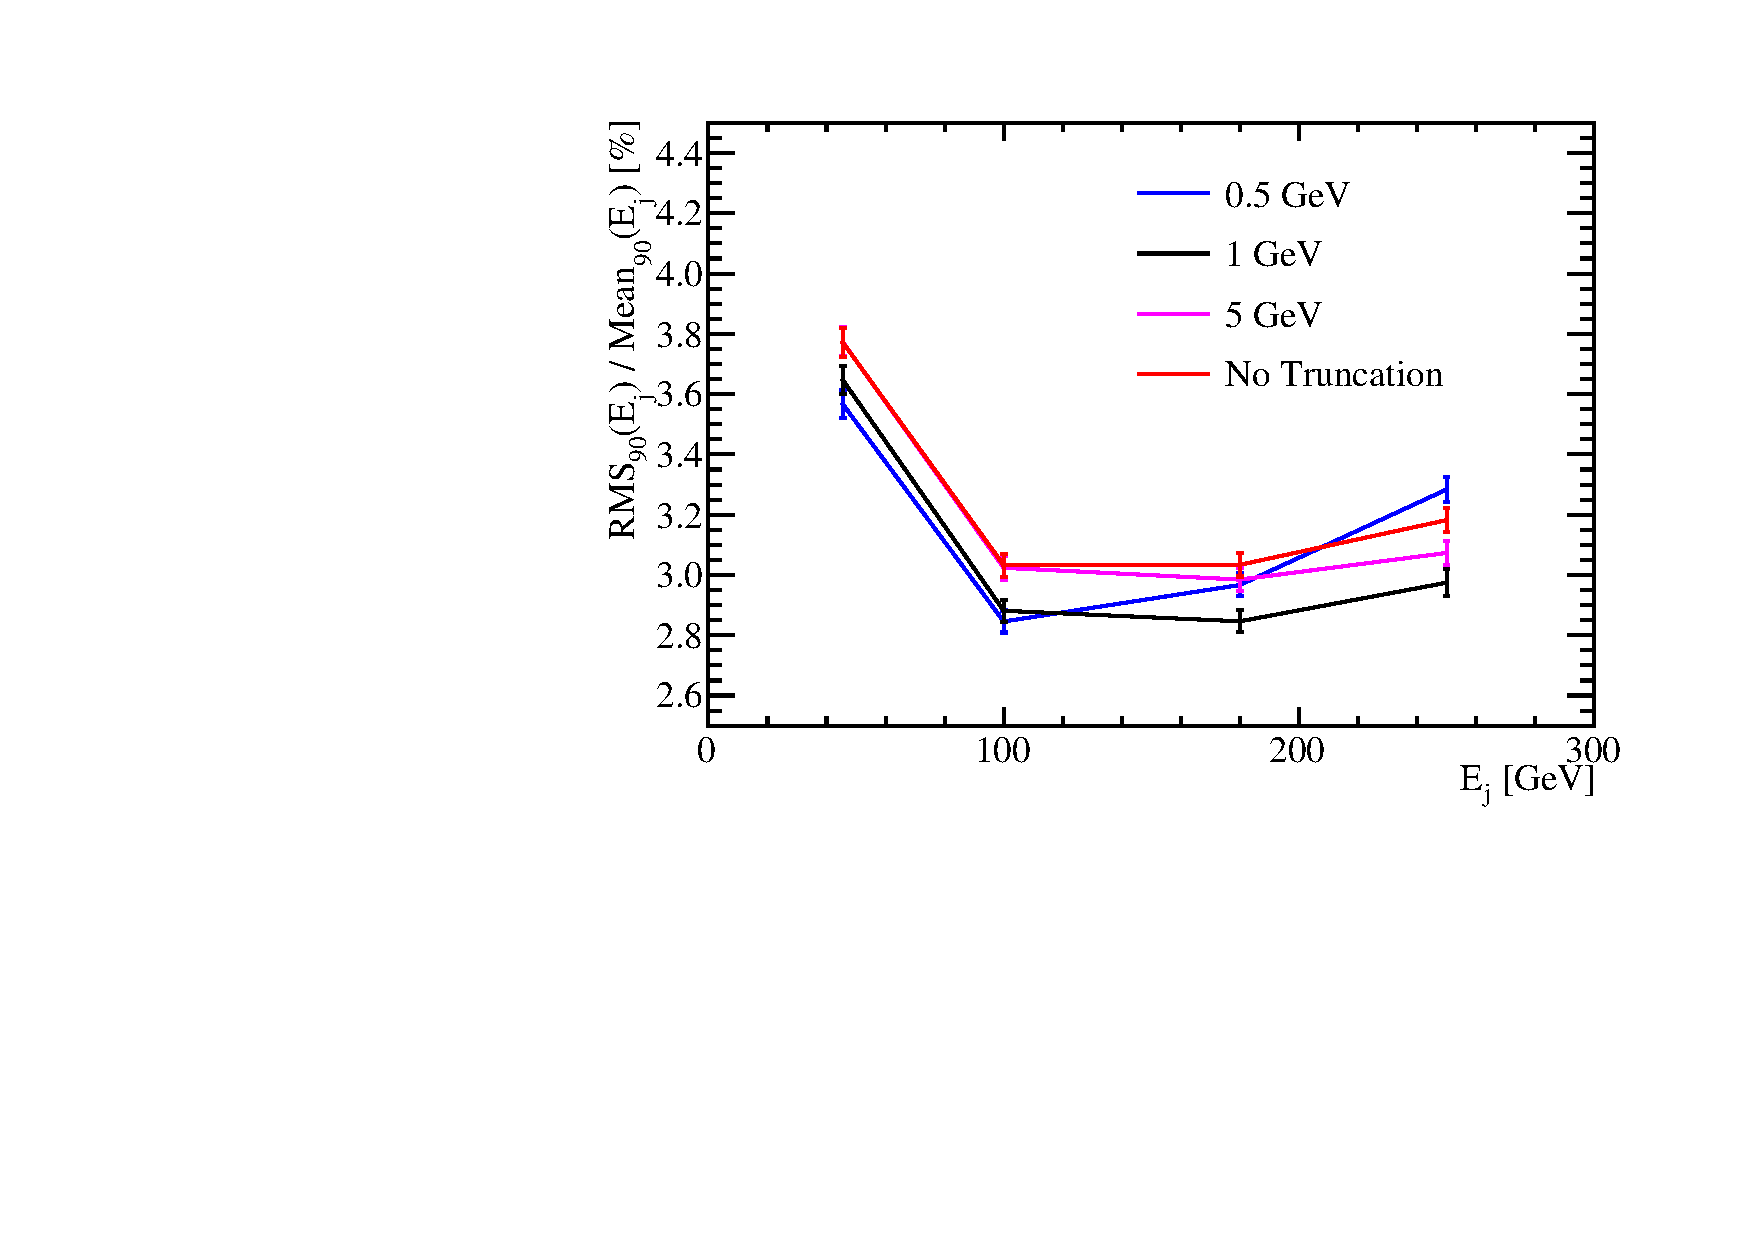
\includegraphics[width=0.5\textwidth]{EnergyEstimators/Plots/CellTruncation/JER_vs_JetEnergy_HCalCellTruncation.pdf}
\caption[The jet energy resolution as a function of jet energy for various HCal hit energy truncations.  The results shown use the nominal ILD detector model, which contains $30\times30 \text{ mm}^{2}$ square scintillator tiles in the HCal.]{The jet energy resolution as a function of jet energy for various HCal hit energy truncations.  The results shown use the nominal ILD detector model, which contains $30\times30 \text{ mm}^{2}$ square scintillator tiles in the HCal.}
\label{fig:jercelltrunc}
\end{figure}

It is clear that a 1~GeV HCal hit energy truncation is beneficial for the performance of the nominal ILD detector model as the jet energy resolution is reduced by roughly $\sim$0.15\% across the jet energy range from 45.5~GeV to 250~GeV.  

%HERE
1)
As this is a significant improvement, this technique is applied for the optimisation studies presented in 
2)
Chapter \ref{chap:detopt} presents an optimisation of the ILD calorimeters and, as it produces a significant improvement in detector performance, the HCal hit energy truncation is used for these simulations.   
3)
Included in these studies is an optimisation of the HCal cell size and, as the average number of particles passing through each calorimeter hit depends on the cell size, the truncation used for each detector model has to be tailored to for cell size considered.  

While it is challenging to determine the optimal truncation to use for any given detector model, it is clear that applying an appropriate truncation produces significant improvement in detector performance.  Therefore, for the optimisation studies presented in chapter \ref{chap:detopt} this form of novel energy estimator is applied.  The optimal truncation for each detector model considered in that study was determined by performing the reconstruction using range of HCal hit energy truncations and quoting the optimal performance.  The HCal hit energy truncations considered in the optimisation study were 0.5, 0.75, 1, 1.5, 2, 5 and 10~GeV.  For the HCal cell size study the truncation used for the 10, 20, 30, 40, 50 and 100~mm cell size detector was 0.5, 0.75, 1, 1.5, 2 and 5~GeV respectively, for the tungsten HCal options the truncation used was 5~GeV and for all other options the truncation used was 1~GeV.  This optimisation has a significant impact on detector optimisation, which can be seen by comparing the jet energy resolutions obtained when using the optimised cell truncation and a fixed 1~GeV truncation, shown in figure \ref{fig:jerhcalcellopt}.  Without this optimisation of hit energy truncation the significance of the HCal cell size is overinflated and could lead to a misinformed detector design choice.  

\begin{figure}[h!]
\subfloat[]{\label{fig:jerhcalcelloptgoodtrunc}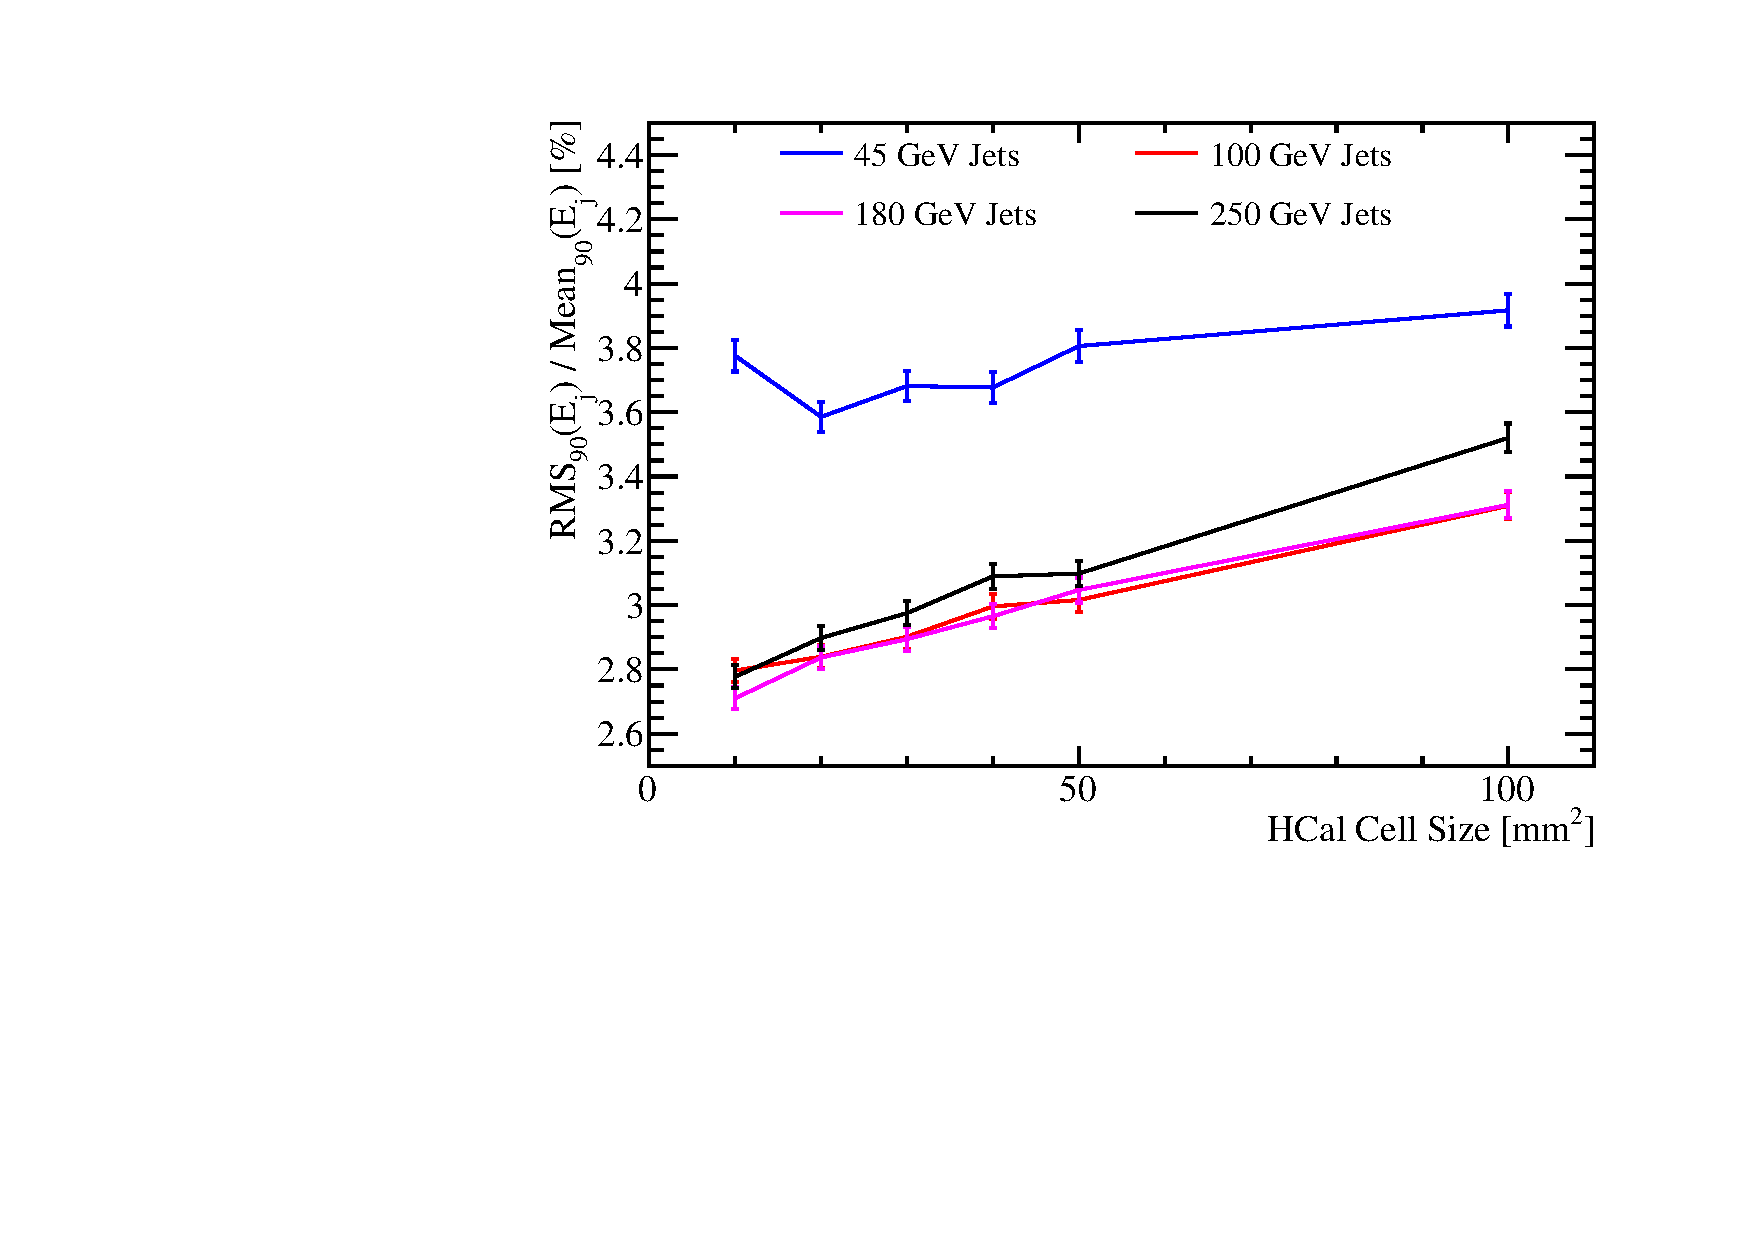
\includegraphics[width=0.5\textwidth]{OptimisationStudies/Plots/JetEnergyResolutions/JER_vs_HCalCellSize.pdf}}
\subfloat[]{\label{fig:jerhcalcelloptbadtrunc}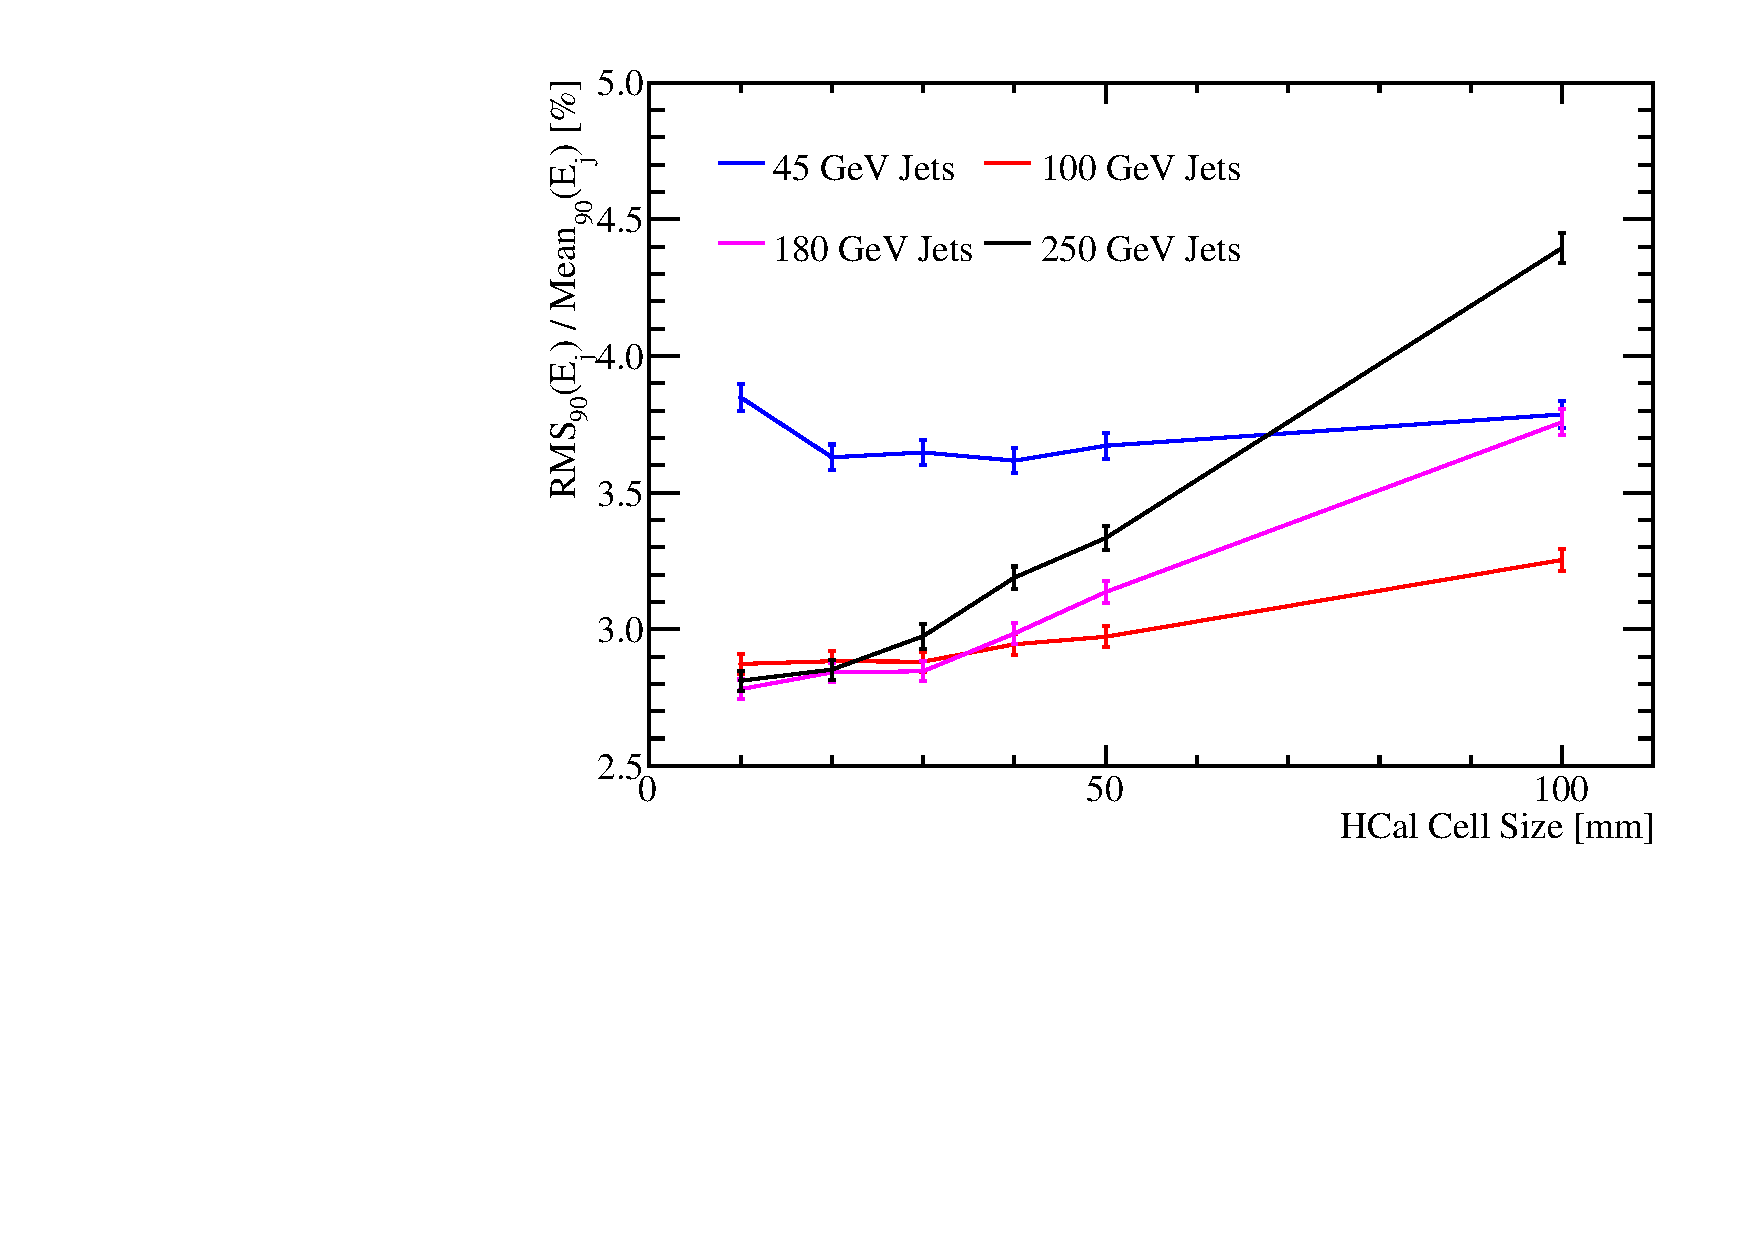
\includegraphics[width=0.5\textwidth]{EnergyEstimators/Plots/CellTruncation/JER_vs_HCalCellSizeBadTruncation.pdf}}
\caption[The jet energy resolution as a function of HCal cell size using a HCal hit energy truncation that is \protect\subref{fig:jerhcalcelloptgoodtrunc} optimised and \protect\subref{fig:jerhcalcelloptbadtrunc} fixed at 1~GeV.]{The jet energy resolution as a function of HCal cell size using a HCal hit energy truncation that is \protect\subref{fig:jerhcalcelloptgoodtrunc} optimised and \protect\subref{fig:jerhcalcelloptbadtrunc} fixed at 1~GeV.}
\label{fig:jerhcalcellopt}
\end{figure}

%========================================================================================

\subsection{Software Compensation}
\label{sec:softcomp}
\subsubsection{Application}
A particle shower produced when a hadron passing through a calorimeter has two components \cite{Wigmans:2000vf}; an electromagnetic shower core, which originates from the production and decay of $\pi^{0}$s and $\eta$s, and a hadronic shower component originating from all other interacting and decaying particles in the shower.  By identifying each of these components in the reconstruction, it is possible to increase the energy of the hadronic hits to give a compensating response and decrease the energy of spuriously high energy hits that come from Landau fluctuations.  The challenge of applying this approach is to identify whether a hit is likely to be hadronic or electromagnetic in nature.  This is done based on the energy density of a hit, with high energy densities likely to be part of the electromagnetic core and low energy densities likely to be part of satellite hadronic hits around the shower core.  An event display showing the energy density of a hadronic shower, where the electromagnetic core can be clearly seen, in a 500~GeV Z$\rightarrow$uds di-jet event can be found in figure \ref{fig:softcompeventdisplay}.  

\begin{figure}[h!]
\subfloat[]{\label{fig:softcompfulleventdisplay}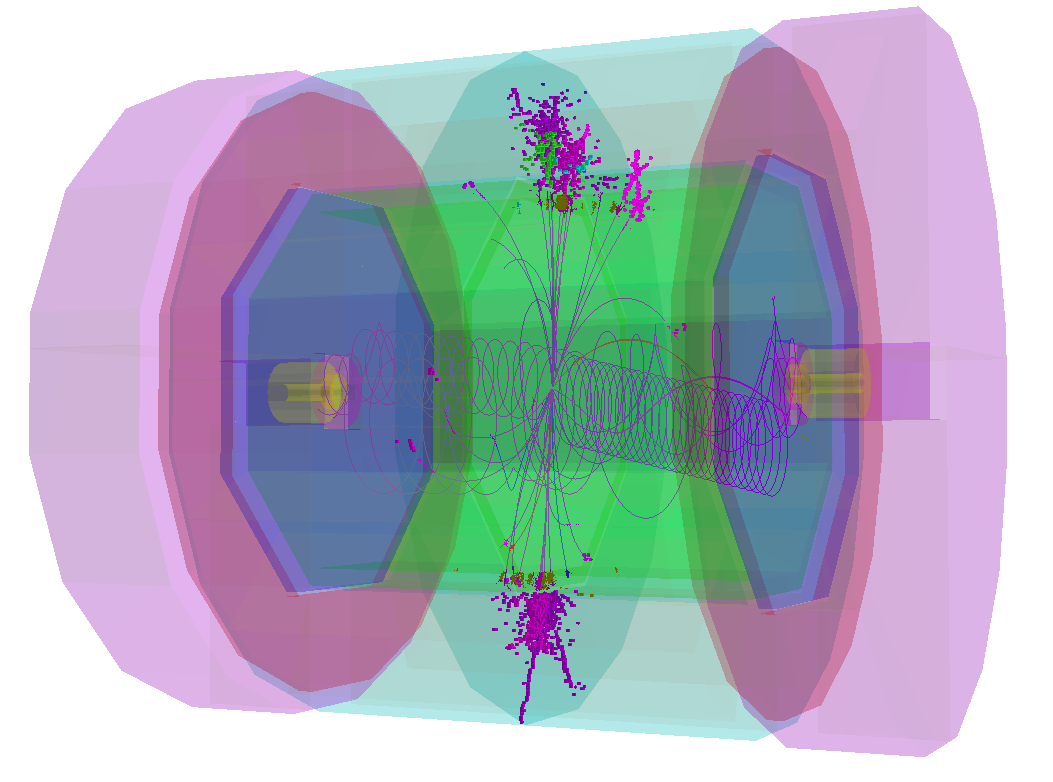
\includegraphics[width=0.5\textwidth]{EnergyEstimators/Plots/SoftComp/VisualDisplay/SoftComp1.png}}
\subfloat[]{\label{fig:softcompclustereventdisplay}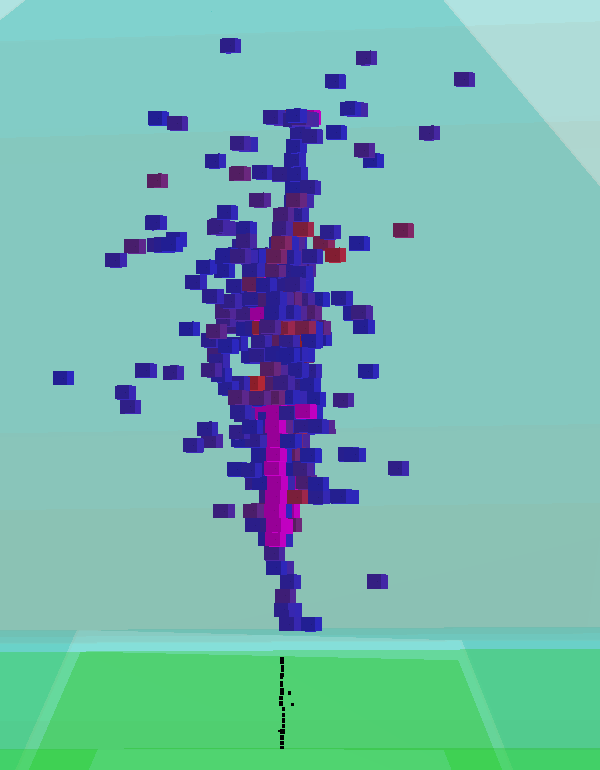
\includegraphics[width=0.3\textwidth]{EnergyEstimators/Plots/SoftComp/VisualDisplay/SoftComp3.png}}
\caption[An event display for a 500~GeV Z$\rightarrow$uds di-jet event reconstructed using the nominal ILD detector.  \protect\subref{fig:softcompfulleventdisplay} The full event environment.  \protect\subref{fig:softcompclustereventdisplay} A single hadronic cluster from the same event where shading indicates the energy density in the HCal.  High energy density cells are coloured red, while lower energy density cells are coloured blue.  All ECal hits are shaded black.  The high energy density electromagnetic core of the selected hadronic cluster is clearly visible.]{An event display for a 500~GeV Z$\rightarrow$uds di-jet event reconstructed using the nominal ILD detector.  \protect\subref{fig:softcompfulleventdisplay} The full event environment.  \protect\subref{fig:softcompclustereventdisplay} A single hadronic cluster from the same event where shading indicates the energy density in the HCal.  High energy density cells are coloured red, while lower energy density cells are coloured blue.  All ECal hits are shaded black.  The high energy density electromagnetic core of the selected hadronic cluster is clearly visible.}
\label{fig:softcompeventdisplay}
\end{figure}

An additional layer of sophistication in this approach is the weights that are applied vary as a function of the uncompensated cluster energy, $E_{\text{Raw}}$, as well as the hit energy density, $\rho^{i}$.  This is to account for any changes to the distribution of calorimeter hit energy densities as the total shower energy is varied.  For example, the fraction of hits in a hadronic shower that are electromagnetic in nature increases as the total energy of the hadronic shower increases \cite{Wigmans:2000vf}.  Therefore, as the total shower energy increases a smaller fraction of hits will require weights greater than one as there are less fully hadronic hits in the shower than at low energies.  The highly segmented calorimeters used at the linear collider experiment will give excellent spatial resolution for individual particle showers, which enables precise mapping of the calorimeter hits to different shower components.  This allows the linear collider to employ this software compensation technique with greater effectiveness than was possible for previous collider experiments.  

In terms of the parameterisation introduced in equation \ref{equ:compensation}, the weights used for this technique are \cite{Adloff:2012gv}
%
\begin{equation}
\omega(E_{\text{Raw}}, \rho) = p_{1}(E_{\text{Raw}}) \times exp(p_{2}(E_{\text{Raw}}) \times \rho) + p_{3}(E_{\text{Raw}}) \\
p_{1} = p_{11} + p_{12} \times E_{\text{Raw}} + p_{13} \times E_{\text{Raw}}^{2} \\
p_{2} = p_{21} + p_{22} \times E_{\text{Raw}} + p_{23} \times E_{\text{Raw}}^{2} \\
p_{3} = \frac{p_{31}}{p_{32} + exp(p_{33} \times E_{\text{Raw}})}\text{ ,}
\label{equ:softcompweight}
\end{equation}
\noindent where $p_{ij}$ are trained parameters and
\begin{equation}
E_{Raw} & = \sum_{ECal \text{ } hits \text{, }i} E^{i}_{ECal} +\sum_{HCal \text{ } hits \text{, }i} E^{i}_{HCal} \text{ .}
\end{equation}
%
\noindent The parameters $p_{ij}$ are determined by performing a $\chi^{2}$ fit of the software compensated cluster energy to the MC energy for samples of $K^{0}_{L}$ ranging from 10 to 100~GeV in steps of 10~GeV.  Using the fitted parameters obtained for the nominal ILD detector, $p_{1}$, $p_{2}$ and $p_{3}$ as a function of $E_{\text{Raw}}$ is shown in figure \ref{fig:softcompparams} and $\omega(E_{\text{Raw}}, \rho)$ as a function of $\rho$ for selected values of $E_{\text{Raw}}$ is shown in figure \ref{fig:softcompweights}.  Figure \ref{fig:softcompweights} shows that the high energy density hits are being reduced in energy to compensate for the effects of Landau fluctuations, while the low energy density hits are being increased in weight to compensate for the invisible energy component found in hadronic showers.  Furthermore, the weights vary as a function of the raw hadronic shower energy to account for the changing energy density topology of hadronic showers with increasing shower energy.

\begin{figure}[h!]
\subfloat[]{\label{fig:softcompparam1}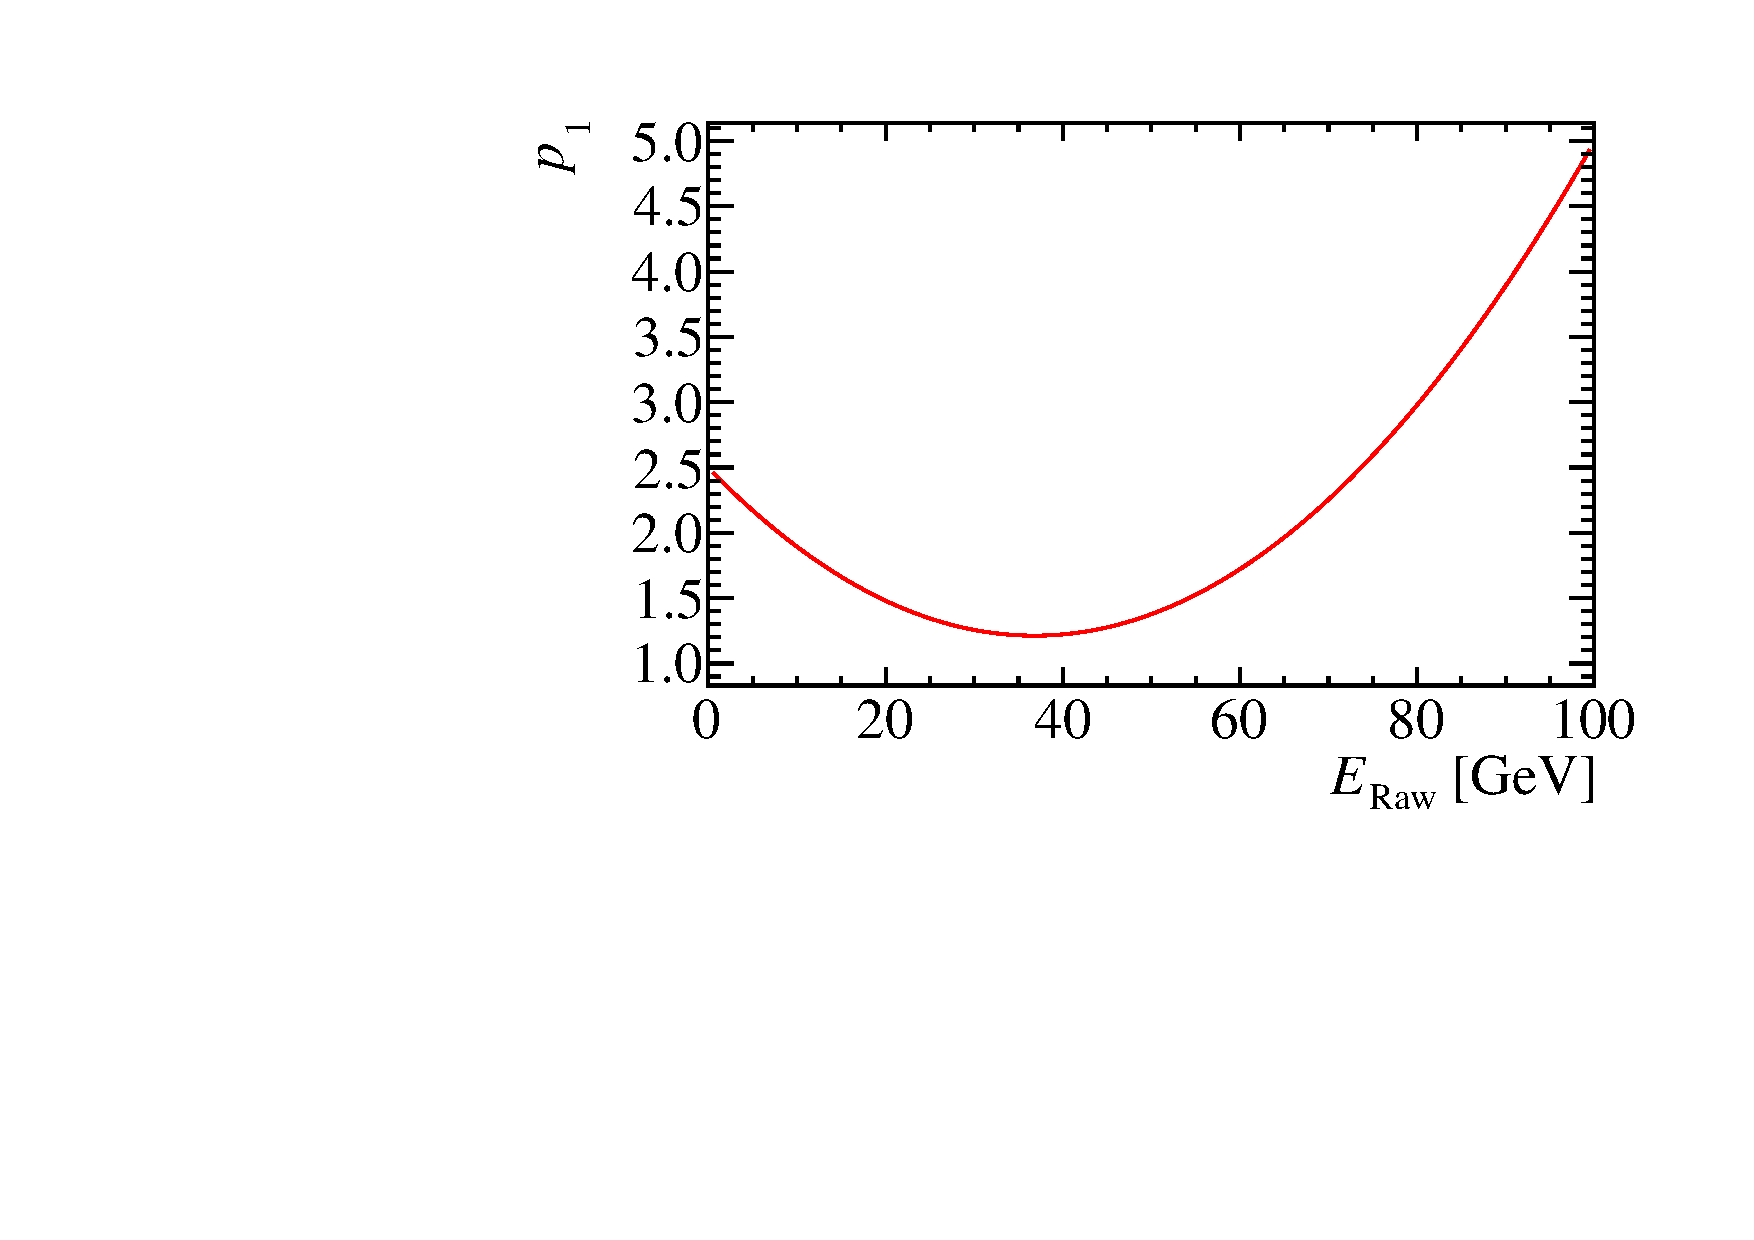
\includegraphics[width=0.33\textwidth]{EnergyEstimators/Plots/SoftComp/Weights/SoftwareCompensationParam1.pdf}}
\subfloat[]{\label{fig:softcompparam2}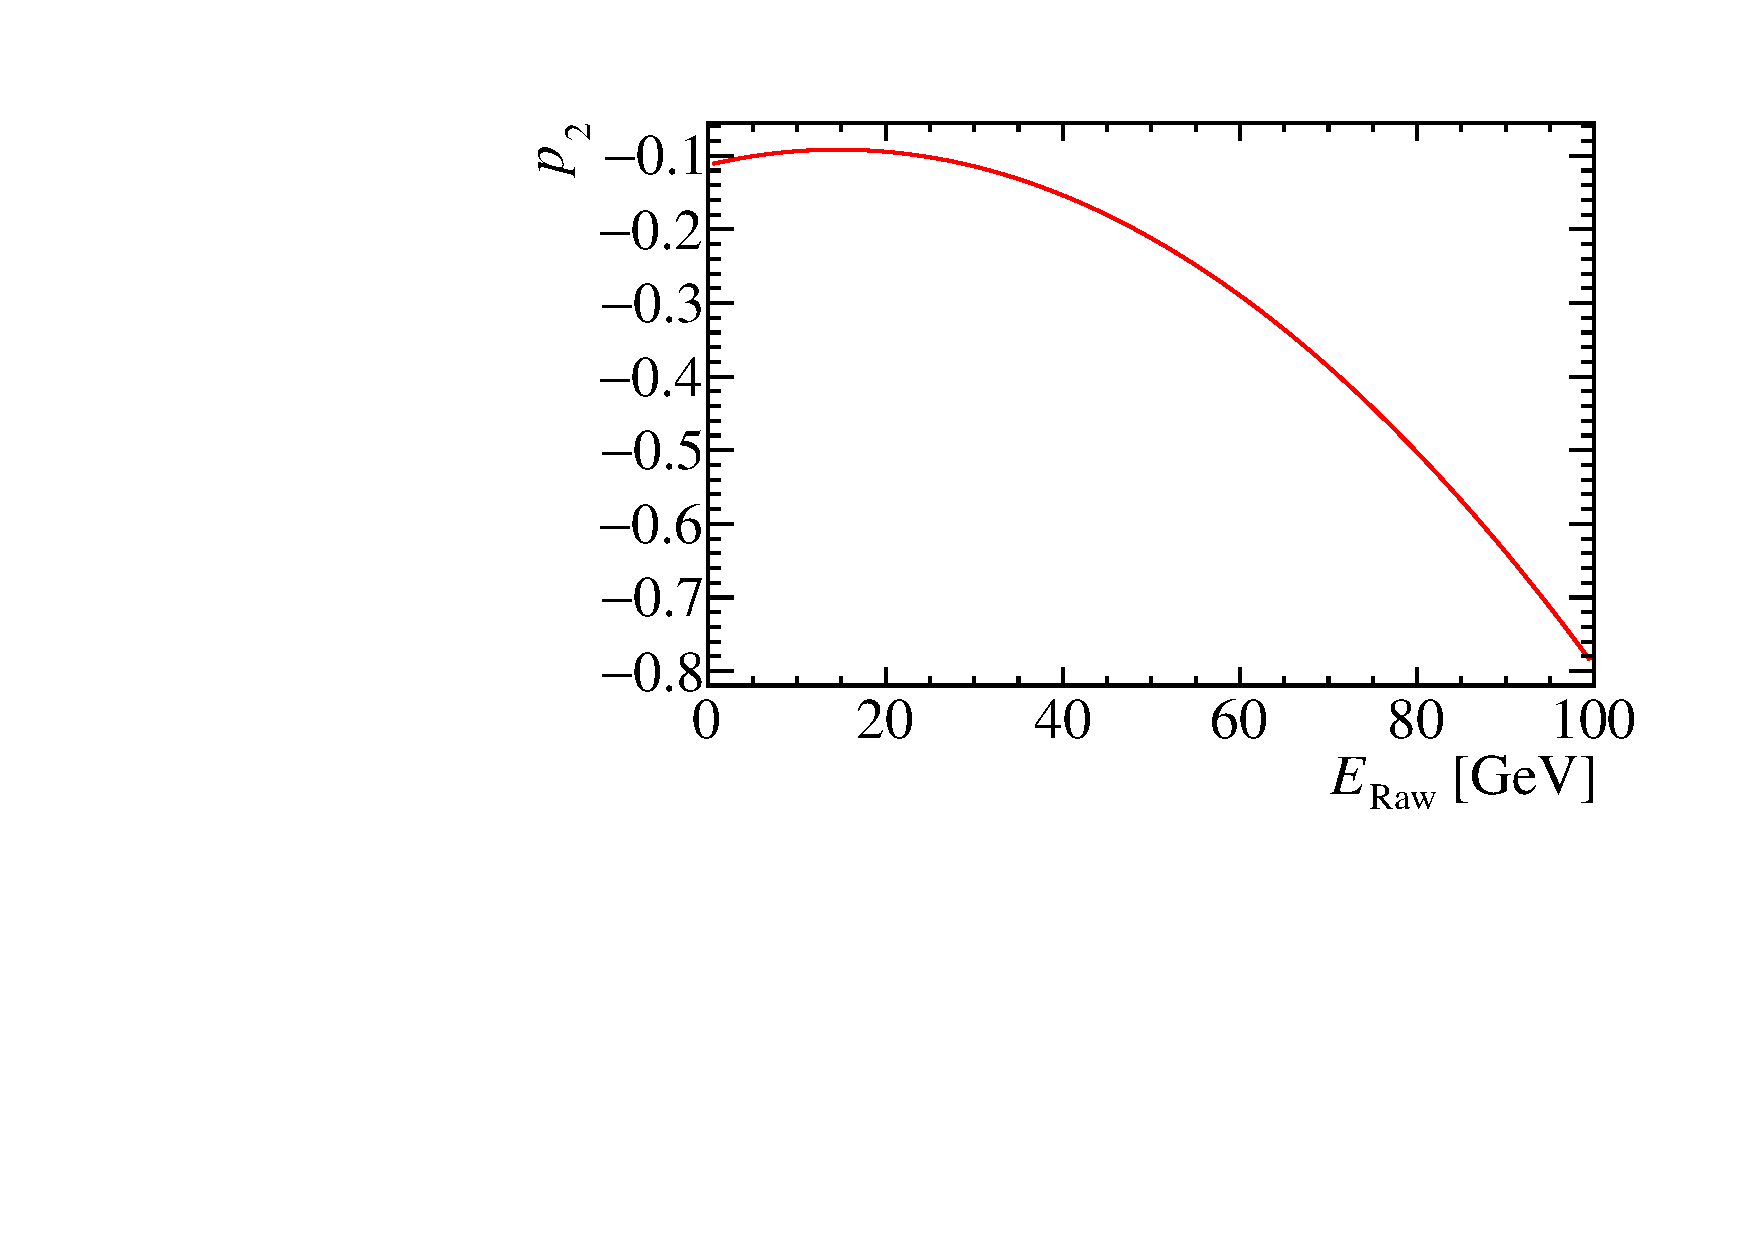
\includegraphics[width=0.33\textwidth]{EnergyEstimators/Plots/SoftComp/Weights/SoftwareCompensationParam2.pdf}}
\subfloat[]{\label{fig:softcompparam3}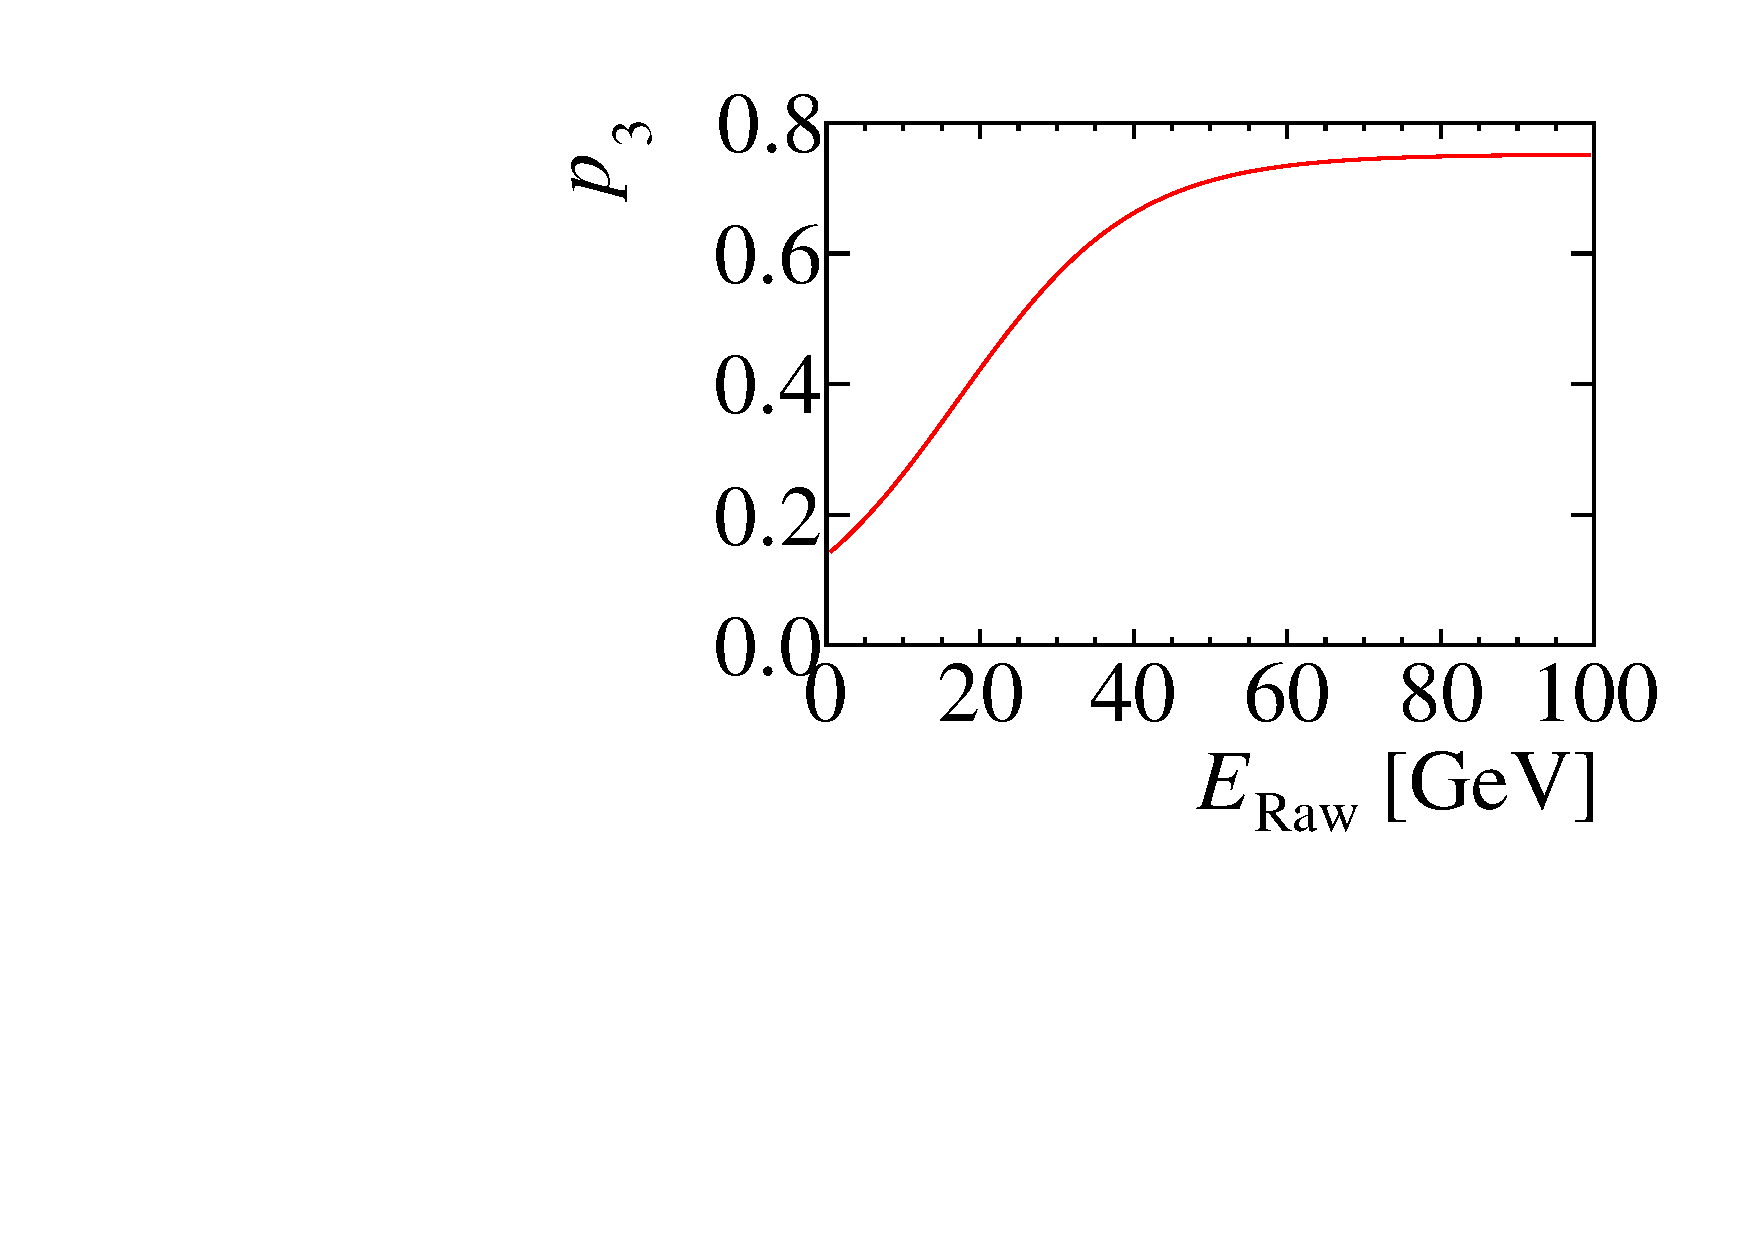
\includegraphics[width=0.33\textwidth]{EnergyEstimators/Plots/SoftComp/Weights/SoftwareCompensationParam3.pdf}}
\caption[Parameters used in software compensation weight determination as a function of $E_{\text{Raw}}$.]{Parameters used in software compensation weight determination as a function of $E_{\text{Raw}}$.}
\label{fig:softcompparams}
\end{figure}

\begin{figure}[h!]
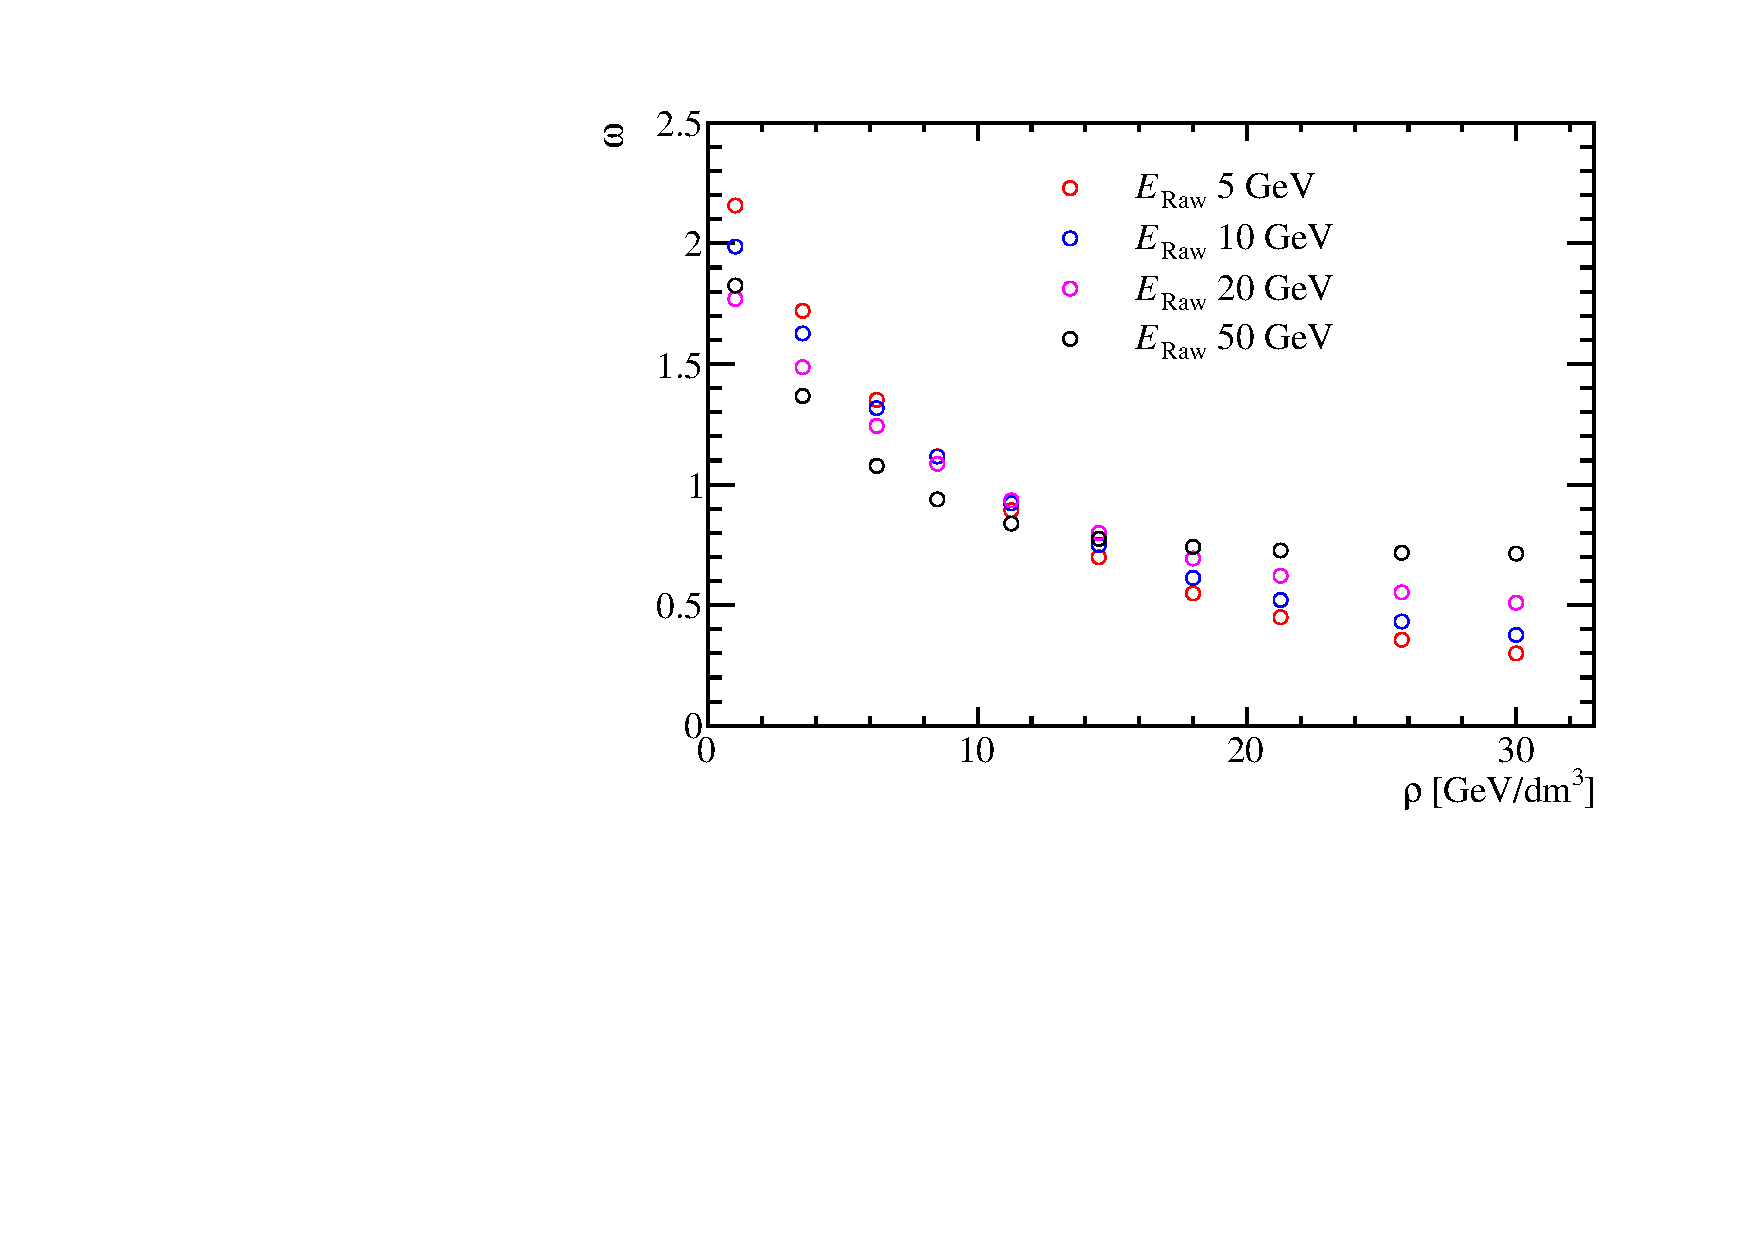
\includegraphics[width=0.5\textwidth]{EnergyEstimators/Plots/SoftComp/Weights/SoftwareCompensationWeights.pdf}
\caption[The software compensation weight applied to a calorimeter hit as a function of calorimeter hit energy density for various cluster energies.]{The software compensation weight applied to a calorimeter hit as a function of calorimeter hit energy density for various cluster energies.}
\label{fig:softcompweights}
\end{figure}

This technique is applied in the PandoraPFA framework in the form of an energy correction function, which means whenever the energy of a cluster of hits is considered by PandoraPFA the software compensated energy is used.  Applying software compensation in this way benefits the detector energy resolution in two ways; firstly, the intrinsic energy resolution of the detector improves and secondly, the confusion contribution to the energy resolution is reduced.

As software compensation only modifies the energy of HCal hits there is freedom to apply further energy corrections to the ECal hits.  Applying the Clean Clusters logic, described in section \ref{sec:legacycorrections}, to the ECal hits alongside software compensation was found to be beneficial to the jet energy resolution.  Therefore, the application of software compensation within PandoraPFA implicitly involves the application of the Clean Clusters logic to the ECal hits.  

Software compensation was trained using a maximum $K^{0}_{L}$ energy of 100~GeV, therefore, it is only applied to clusters where $E_{\text{Raw}} < 100$~GeV as sensible behaviour outside this range cannot be ensured.  While it would be possible to modify the energy range of the training sample to go to higher energies, hadronic clusters with energy greater than 100~GeV will be rare at the ILC like energies considered here.

%========================================================================================

\subsubsection{Context: Legacy Energy Corrections}
\label{sec:legacycorrections}
Before examining the impact of software compensation on detector performance is it necessary to address the 'legacy' energy corrections that are used by default in PandoraPFA.  The three energy correction that were in use prior to the development of software compensation are:

\begin{itemize}
\item \textbf{HCal hit energy truncation}, the details of which can be found in section \ref{sec:hcalcelltruncation}.
\item \textbf{Clean Clusters}.  This algorithm checks to see whether the energy measured within a calorimeter hit is anomalously high.  Anomalously high energy hits are defined as hits where the energy contained within the hit is greater than 10\% of the energy of the cluster that the hit has been associated to.  If a hit is deemed to have an anomalously high energy and if this energy is above a threshold (0.5~GeV) the hit energy used by PandoraPFA is modified.  The updated hit energy is taken as the average hit energy in the calorimeter layers immediately before and after the layer containing the high energy hit.    
\item \textbf{Scale Hot Hadrons}.  This algorithm calculates the average number of MIP equivalent particles passing through each calorimeter hit in a cluster.  If this number is larger than a given value, default 15 MIPs per hit, the cluster energy is rescaled to give a lower average number of MIPs per hit, default is 5 MIPs per hit.  
\end{itemize}

Each of these energy corrections help to deal with the effects of spuriously high energy hits the origin of which is described in section \ref{sec:hcalcelltruncation}.  However, the algorithms are simplistic and software compensation is expected to give far better results than these 'legacy' options.  The optimisation studies presented in section \ref{chap:detopt} use all three of these legacy options simultaneously, which was the default behaviour for PandoraPFA when the studies were undertaken.  The new default behaviour in PandoraPFA is to use software compensation.

%========================================================================================

\subsubsection{Results: Energy Resolution}
\label{sec:softcomper}
The energy resolution as a function of the MC energy for single $K^{0}_{L}$ events is shown in figure \ref{fig:ersoftcomp} using various energy correction settings.  When comparing the energy resolution given by software compensation to that obtained using no energy corrections, it can be seen that software compensation offers a gain of $\approx 2 \%$ in energy resolution across the energy range considered.  The uniformity of this improvement is encouraging, indicating software compensation is achieving a compensating calorimeter response across this wide range of energies.  

Comparing the performance of software compensation to the legacy corrections it can be seen that software compensation gives a better energy resolution across almost the entire range of energies considered.  The only exception to this is around $E_{K^{0}_{L}} \approx 50$~GeV where the performance of software compensation and the legacy corrections are comparable.  By removing the hit truncation from the legacy options it is clear that the changes in energy resolution when using the legacy options are being driven by the hit truncation.  This makes the trend in energy resolution observed using the legacy corrections clear as, at low $K^{0}_{L}$ energies, very few hits are affected by the truncation so the performance is comparable to not using any energy corrections.  At high $K^{0}_{L}$ energies, the truncation is too aggressive and removes energy from hits that are not spuriously high leading to a worsening energy resolution.  Between these two extremes, $E_{K^{0}_{L}} \approx 50$~GeV, the truncation works ideally and the improvement in energy resolution when using the legacy corrections is the largest.  

\begin{figure}[h!]
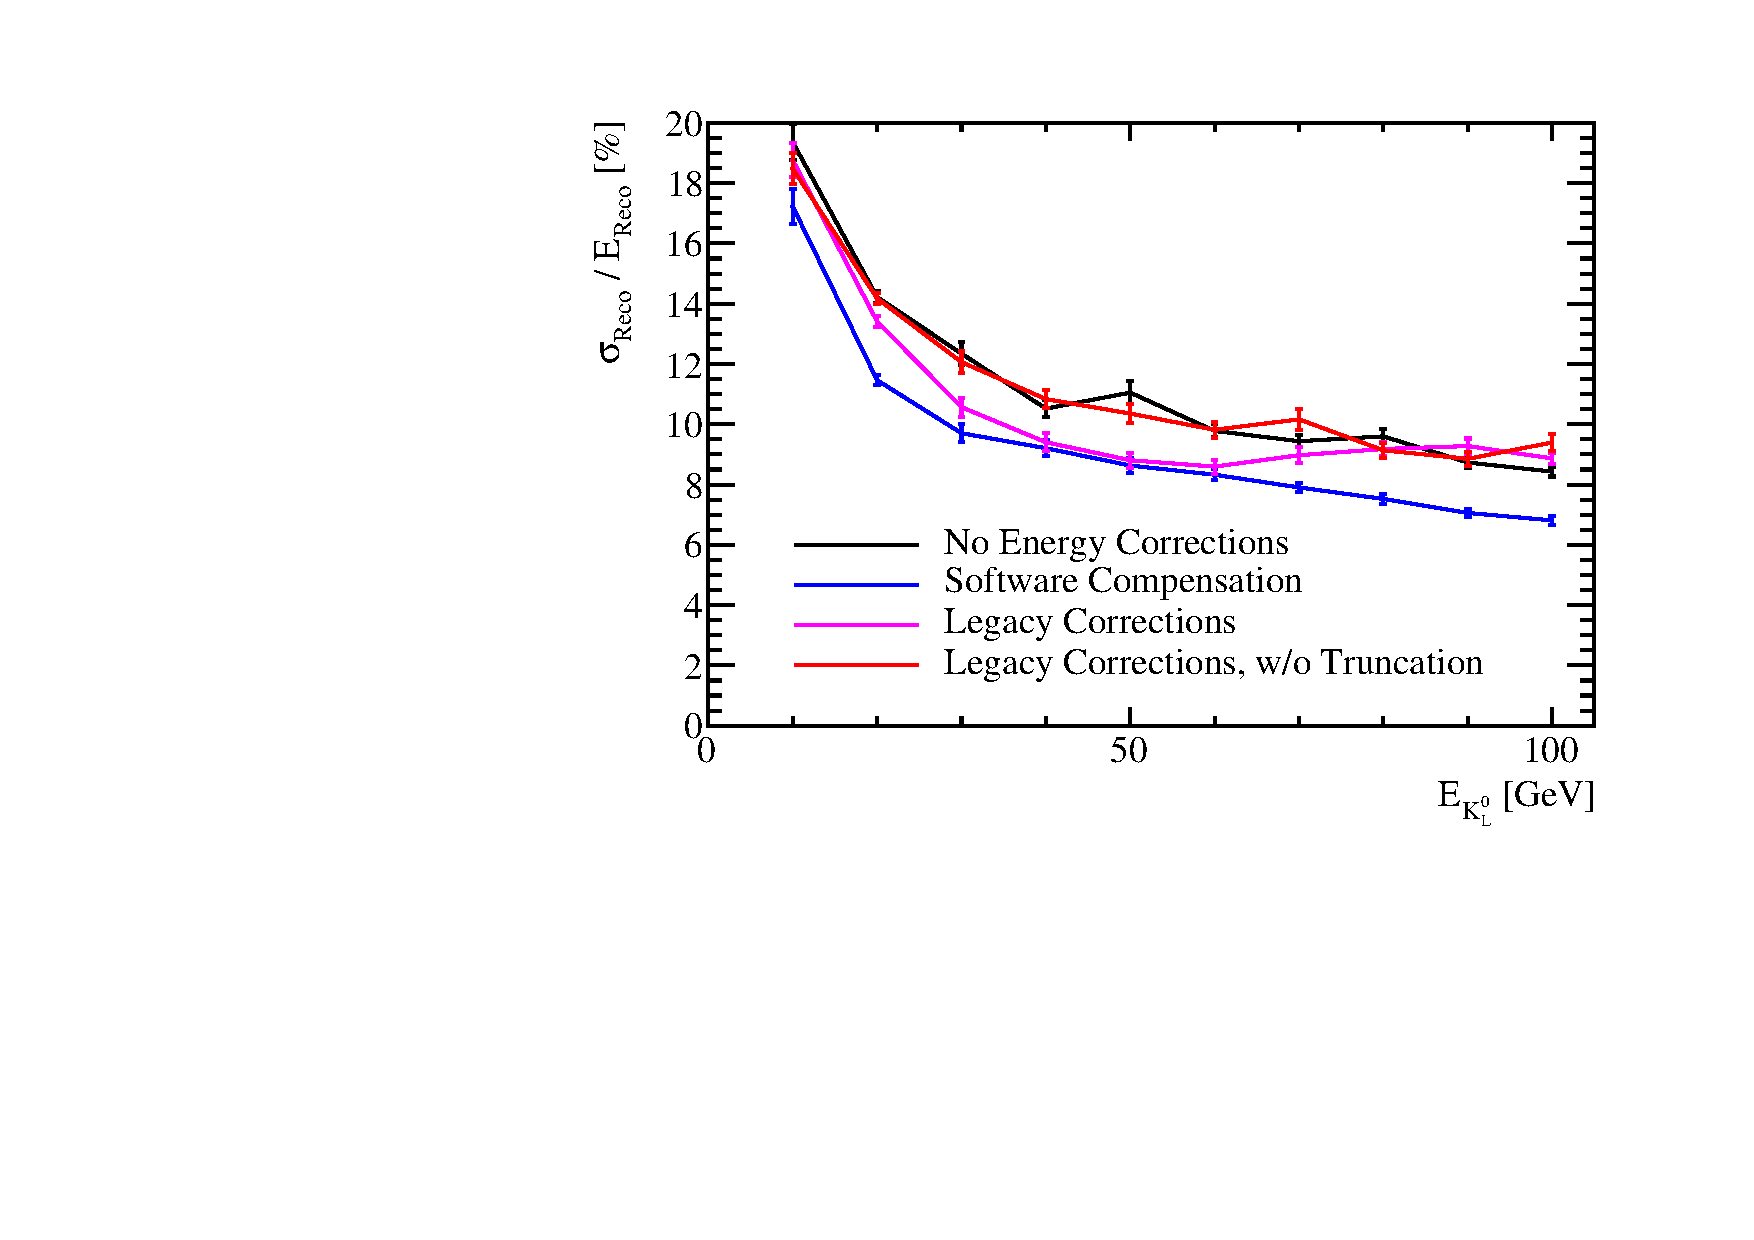
\includegraphics[width=0.5\textwidth]{EnergyEstimators/Plots/SoftComp/EnergyResolution/ER_vs_Kaon0LSoftComp_Kaon0L.pdf}
\caption[The energy resolution as a function of the MC energy for single $K^{0}_{L}$ events using various energy correction settings.  The detector model used was the nominal ILD detector model.]{The energy resolution as a function of the MC energy for single $K^{0}_{L}$ events using various energy correction settings.  The detector model used was the nominal ILD detector model.}
\label{fig:ersoftcomp}
\end{figure}

%========================================================================================

\subsubsection{Results: Jet Energy Resolution}
The improvements in the intrinsic energy resolution of the detector observed when using software compensation will propagate into the reconstruction of jets.  These effects are illustrated by examining the jet energy resolution as a function of jet energy, which is shown in figure \ref{fig:jersoftcomp}.  Again it is clear that software compensation is extremely beneficial to the detector performance as it gives a significant reduction in the jet energy resolution in comparison to using the legacy energy corrections.  

\begin{figure}[h!]
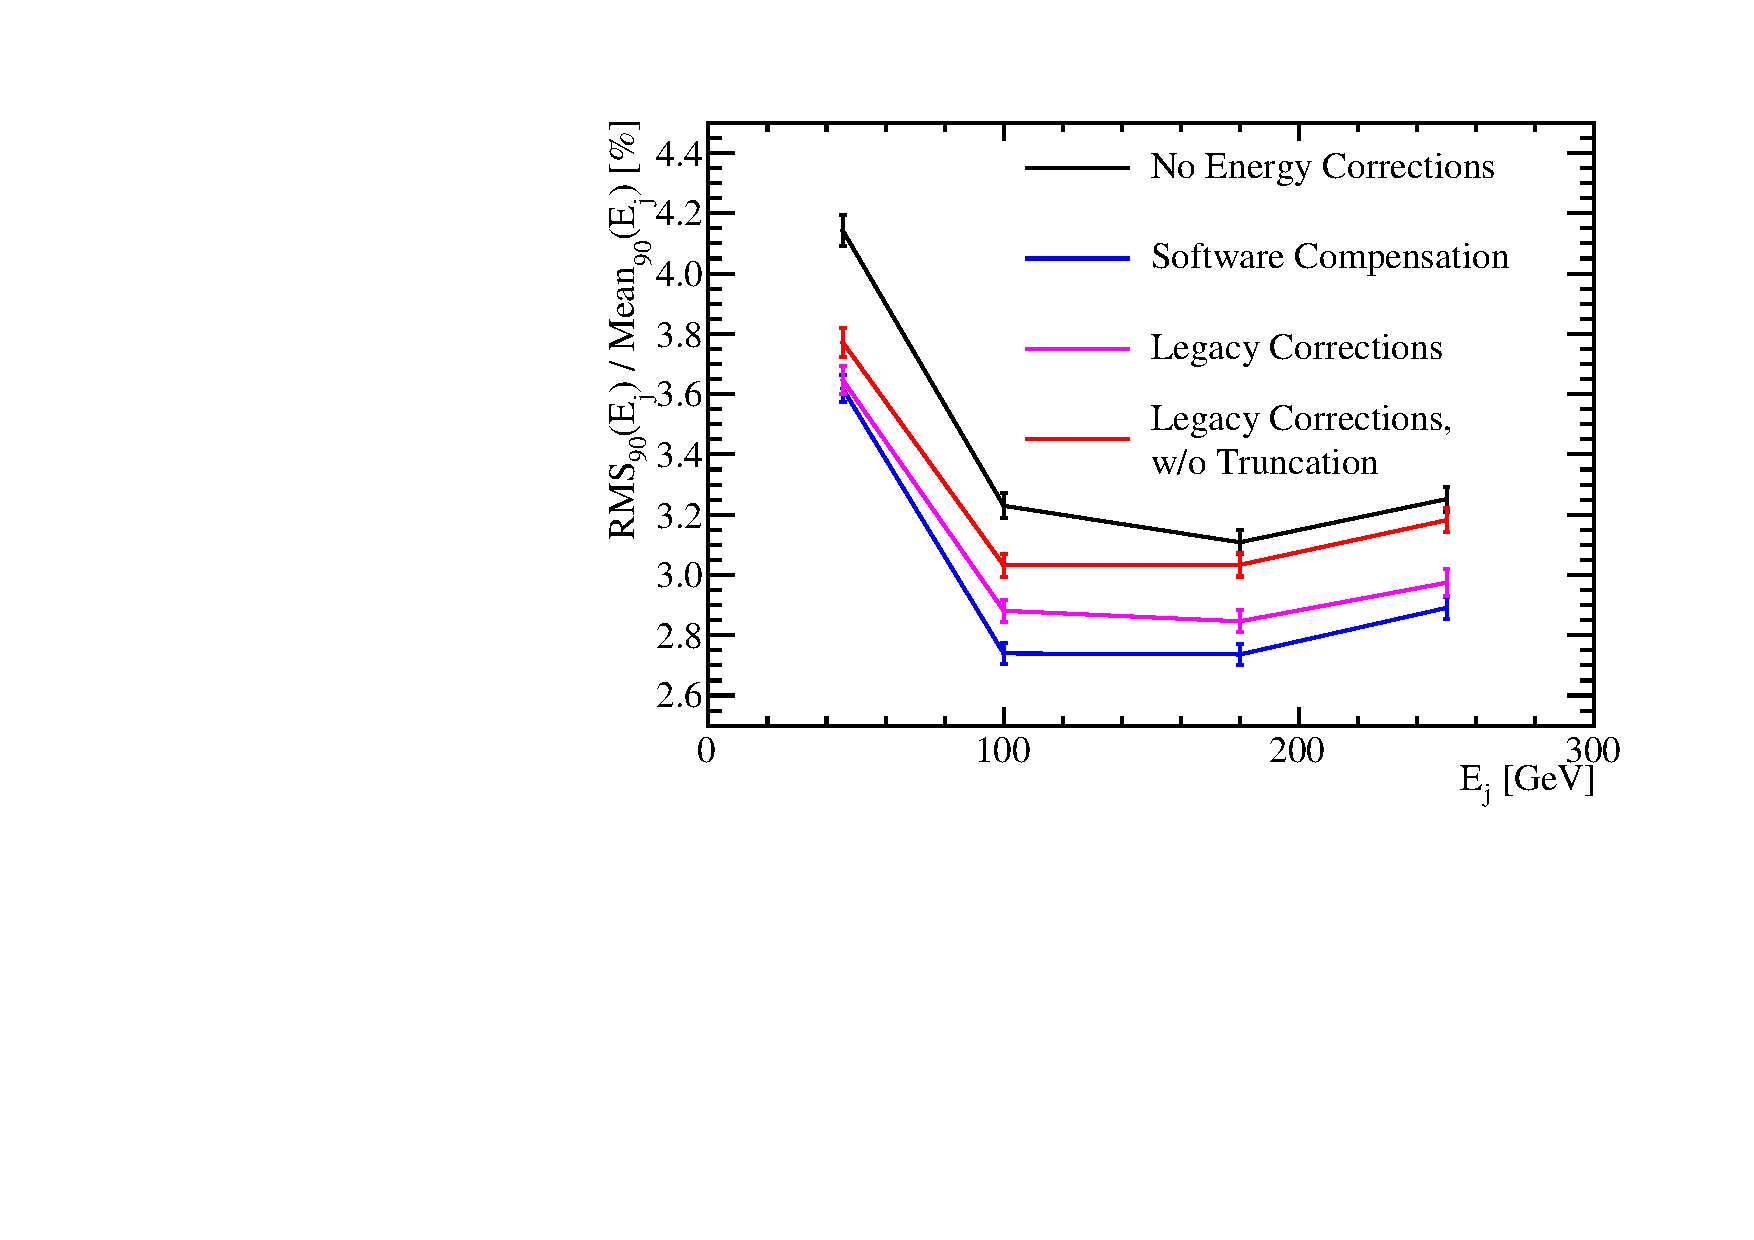
\includegraphics[width=0.5\textwidth]{EnergyEstimators/Plots/SoftComp/JetEnergyResolution/JER_vs_JetEnergy_Default.pdf}
\caption[The jet energy resolution as a function of the jet energy for a variety of different energy correction options.  These results were produced for the nominal ILD detector model.]{The jet energy resolution as a function of the jet energy for a variety of different energy correction options.  These results were produced for the nominal ILD detector model.}
\label{fig:jersoftcomp}
\end{figure}

Further light can be shed on these trends by examining the contributions to the jet energy resolutions from the intrinsic energy resolution and the pattern recognition confusion, which are shown in figure \ref{fig:jerbreakdownsoftcomp}.  The intrinsic energy resolution contribution shows that software compensation is significantly better than all other energy corrections options, which is to be expected from the energy resolution studies presented in section \ref{sec:softcomper}.  Unlike the single particle study there is no jet energy for which the hit truncation matches the performance obtained using software compensation.  This is due to the fact that the energy resolution when using the hit truncation is only comparable to the energy resolution using software compensation for a narrow range of hadronic cluster energies.  As the jet contains a broad spectrum of hadronic cluster energies the performance obtained when using the hit truncation will always be worse than when using software compensation.  When comparing the jet energy resolution for the legacy corrections is again apparent that the term driving the jet energy resolution is the hit truncation.

\begin{figure}[h!]
\subfloat[]{\label{fig:jerbreakdownsoftcomp1}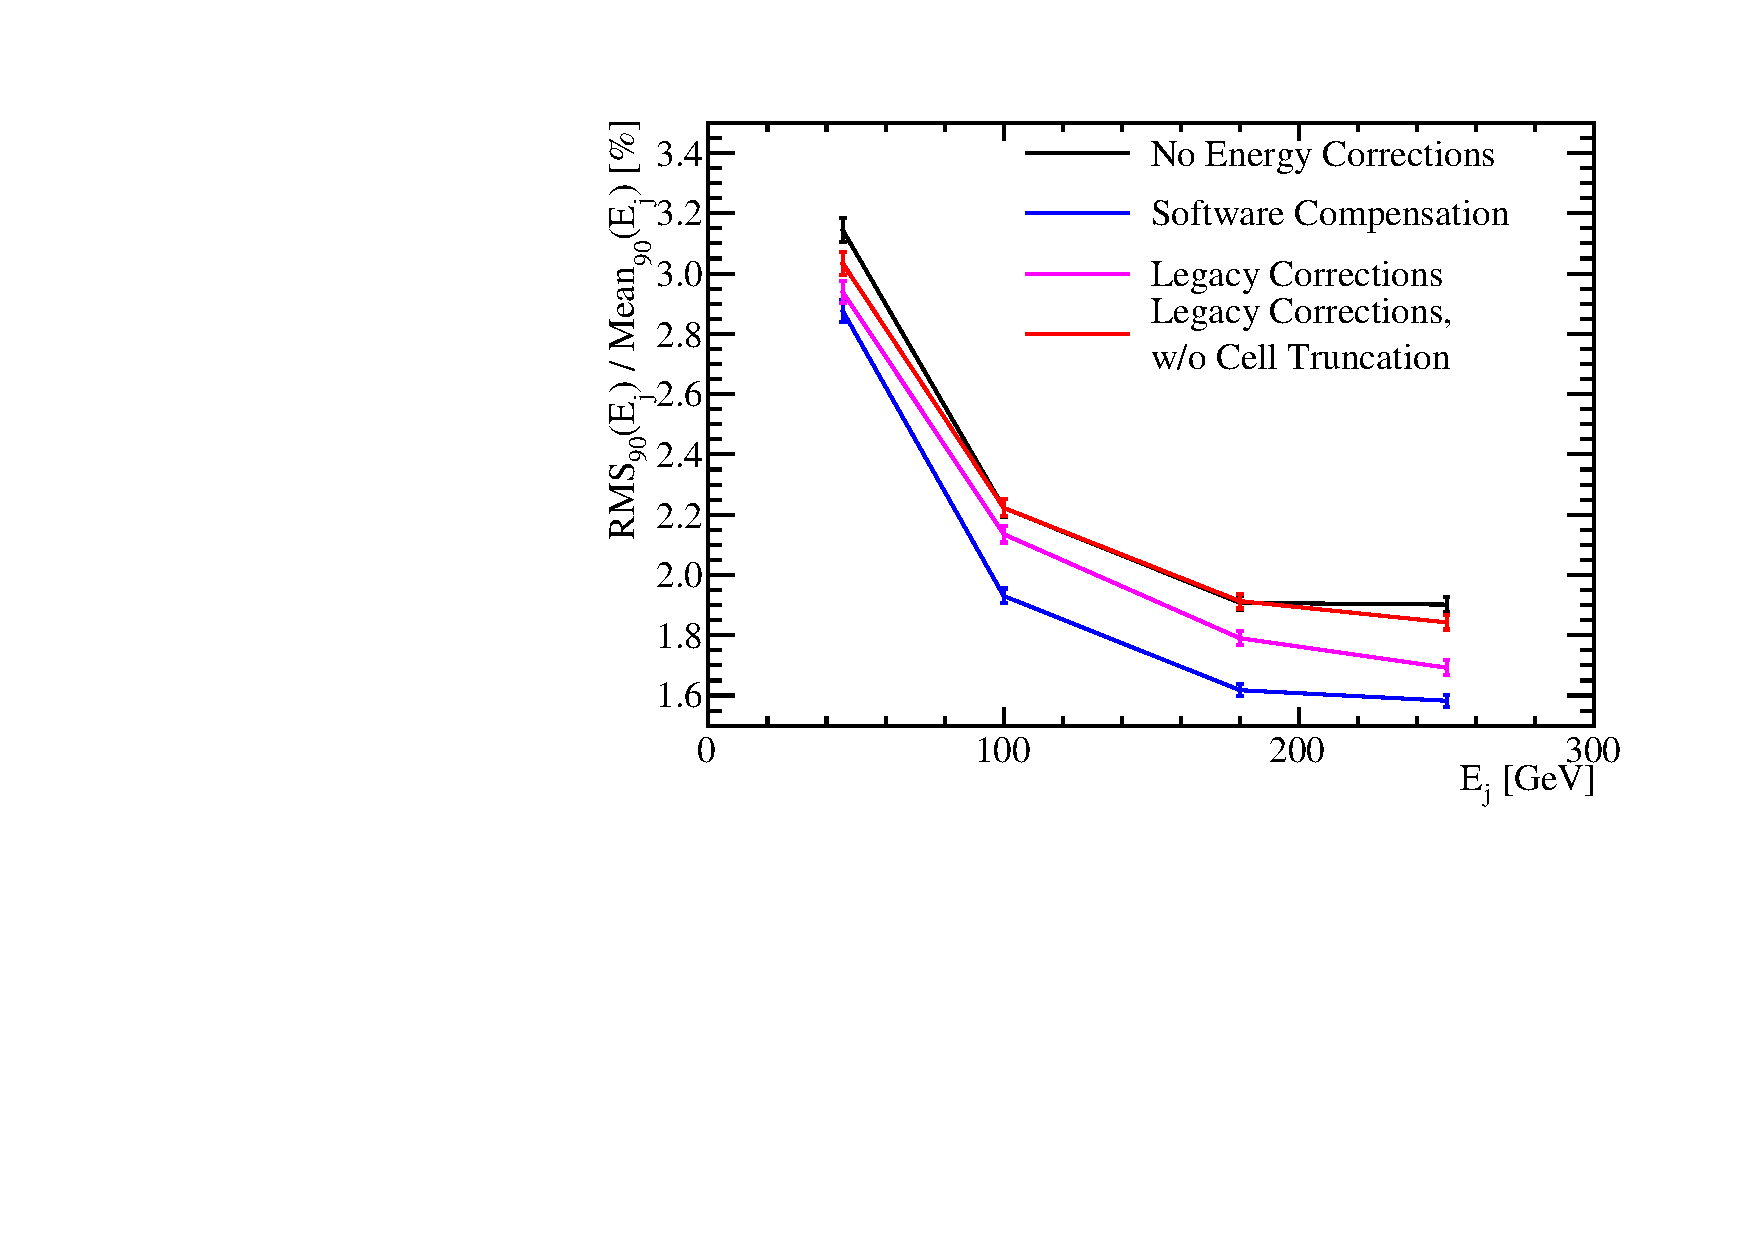
\includegraphics[width=0.5\textwidth]{EnergyEstimators/Plots/SoftComp/JetEnergyResolution/JER_vs_JetEnergy_PerfectPFA.pdf}}
\subfloat[]{\label{fig:jerbreakdownsoftcomp2}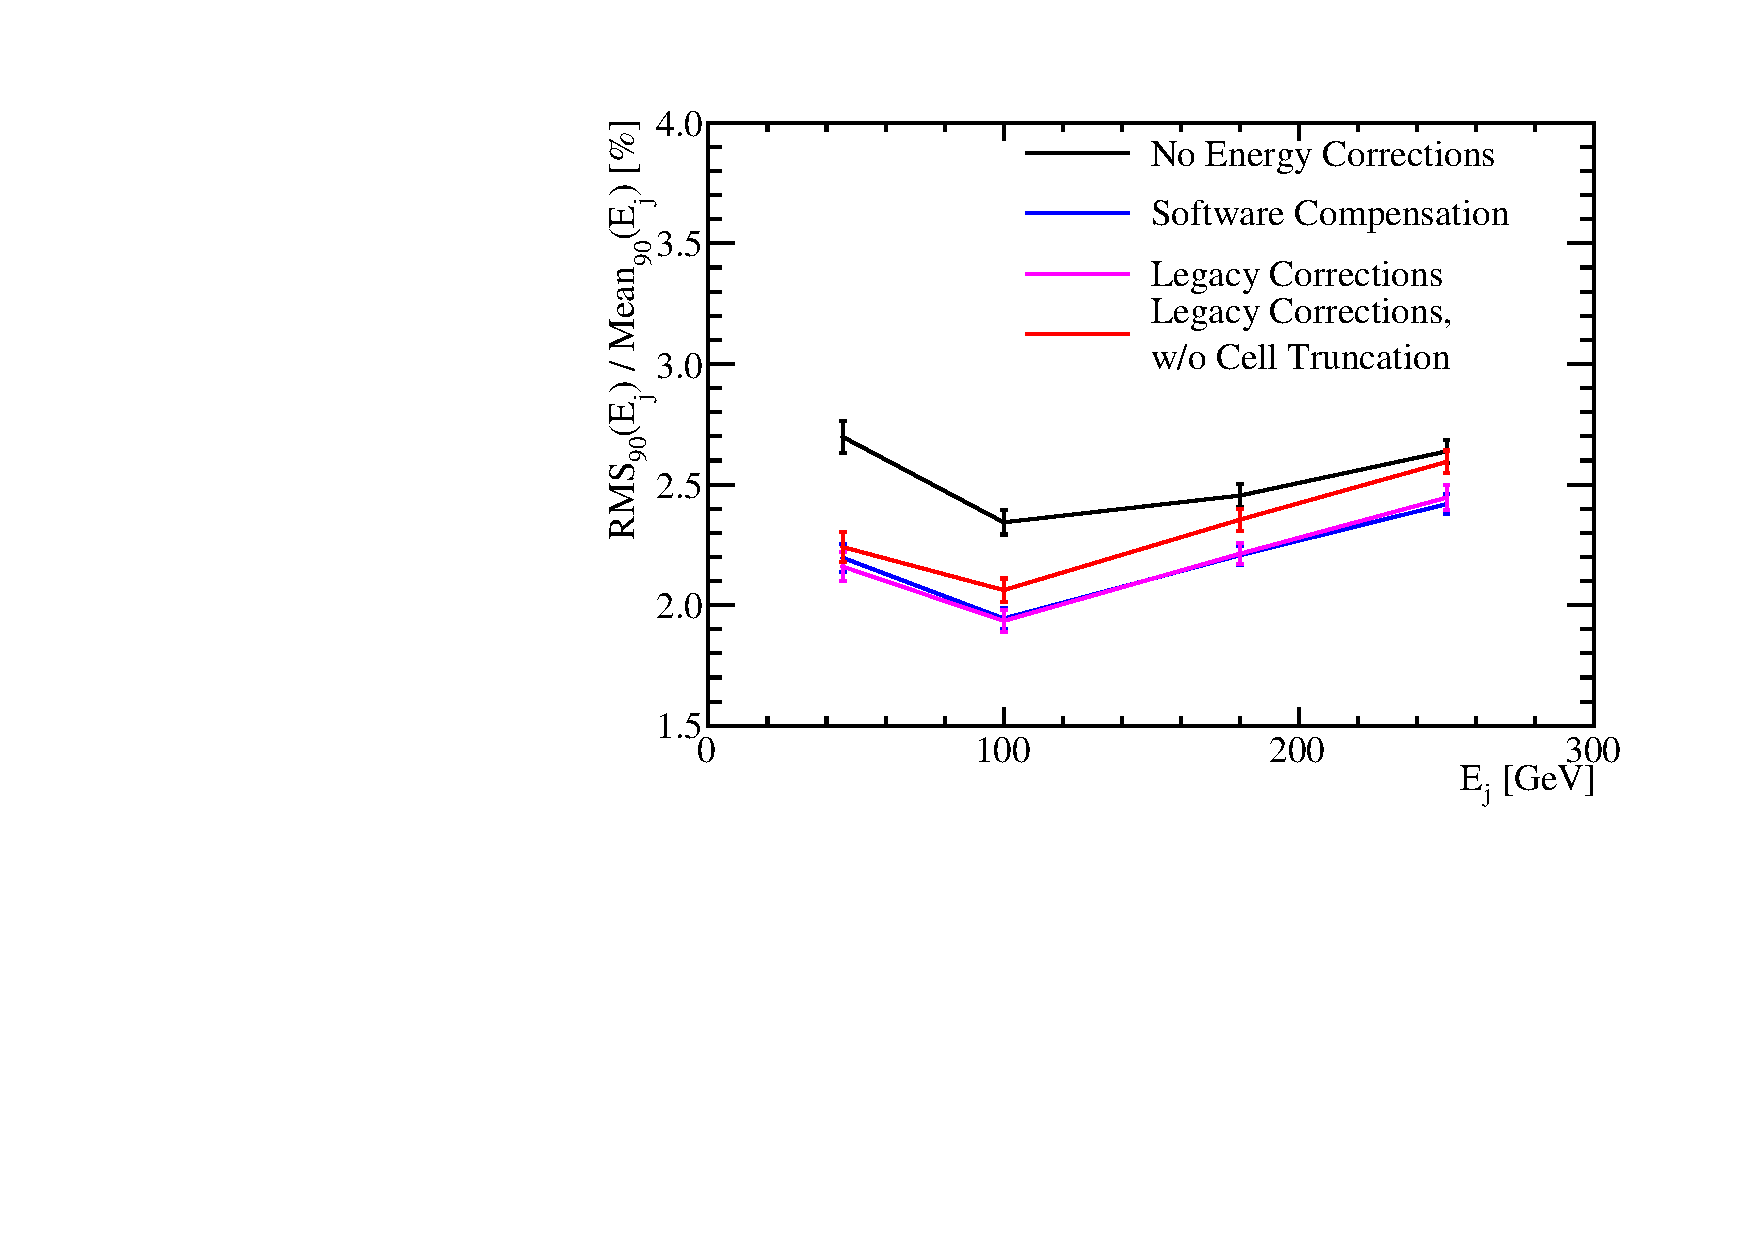
\includegraphics[width=0.5\textwidth]{EnergyEstimators/Plots/SoftComp/JetEnergyResolution/JER_vs_JetEnergy_TotalConfusion.pdf}}
\caption[The contributions to the jet energy resolution as a function of the jet energy for a variety of different energy correction options.  \protect\subref{fig:jerbreakdownsoftcomp1} is the intrinsic energy resolution of the detector and \protect\subref{fig:jerbreakdownsoftcomp2} is the total confusion term.  The quadrature sum of both yields the standard reconstruction performance.  These results were produced for the nominal ILD detector model.]{The contributions to the jet energy resolution as a function of the jet energy for a variety of different energy correction options.  \protect\subref{fig:jerbreakdownsoftcomp1} is the intrinsic energy resolution of the detector and \protect\subref{fig:jerbreakdownsoftcomp2} is the total confusion term.  The quadrature sum of both yields the standard reconstruction performance.  These results were produced for the nominal ILD detector model.}
\label{fig:jerbreakdownsoftcomp}
\end{figure}

The confusion contributions to the jet energy resolution when using software compensation and the legacy corrections are almost identical.  This indicates that the improvement seen in the jet energy resolution when comparing software compensation and the legacy corrections, shown in figure \ref{fig:jersoftcomp}, is being driven by the intrinsic energy resolution.  The hit truncation and software compensation techniques both improve the energy resolution of the hadronic clusters, however, software compensation is far more effective.  

At low jet energies the Clean Clusters and Scale Hot Hadrons energy corrections are beneficial for reducing the confusion contribution, while the hit truncation is largely redundant.  For high jet energies jets this trend is reversed.  As the Clean Clusters and Scale Hot Hadrons energy corrections do not alter the intrinsic energy resolution of the detector, it is clear that they are compensating for failures in the pattern recognition, which occur primarily at low jet energies.  By extracting the Clean Clusters logic, which is the driving term reducing the confusion contribution to the jet energy resolution at low jet energies, and embedding it within the software compensation energy correction, it is possible to obtain exceptional jet energy resolutions that will extend the physics reach of the linear collider detector.  

%========================================================================================
%========================================================================================

\section{Timing Cuts}
The linear collider will operate using a trigger-less readout approach whereby the recorded data for each sub-detector is readout between collisions of $\text{e}^{+}$ and $\text{e}^{-}$ bunches.  The train structure for ILC and CLIC, at their maximum operating energy, is shown in table \ref{table:trainstructure}.  Event selection will proceed through the application of a software trigger.  This involves the identification of any hard interactions, prior to full event reconstruction, and only putting data into the event reconstruction if it is measured within a chosen time window about these interactions.  The recorded time of a calorimeter hit, which is cut on to make the time window for the software trigger, is corrected for straight time-of-flight to the IP.  This ensures that the amount of time particle showers have to develop in the calorimeters is independent of their position in the detector.  As the width of this time window changes, the amount of time particle showers have to develop changes, which will affect the performance of the detector.  

\begin{table}[h!]
\centering
\begin{tabular}{l r r}
\hline
& ILC 500~GeV & CLIC 3 TeV \\
\hline
Electrons per bunch [$10^{10}$] & 2.0 & 0.37 \\
Bunches per train & 2820 & 312 \\
Train repetition rate [Hz] & 5 & 50 \\
Bunch separation [ns] & 308 & 0.5 \\
\end{tabular}
\caption[The train structure for 500~GeV ILC and 3 TeV CLIC \cite{Behnke:2013lya,Linssen:2012hp}.]{The train structure for 500~GeV ILC and 3 TeV CLIC \cite{Behnke:2013lya,Linssen:2012hp}.}
\label{table:trainstructure}
\end{table}

For all choices of time window considered in this study the calibration procedure described in section \ref{sec:overviewcalibration} was applied.  This ensure that the mean of the reconstructed energy distributions will be invariant to changes in the calorimeter timing window as the calibration procedure compensates for any energy losses incurred by truncating the particle shower development time.  

%========================================================================================

\subsubsection{Results: Energy Resolution}
The energy resolution for100~GeV $\gamma$ and 50~GeV $K^{0}_{L}$ events as a function of the timing window applied to the calorimeter hits is shown, for the nominal ILD detector, in figure \ref{fig:ertimingcuts}.  The timing cut makes little difference to the energy resolution of the $\gamma$ events, however, there is a significant decrease in the energy resolution for the neutral hadrons.  This is to be expected as electromagnetic showers develop far more rapidly than their hadronic counterparts \cite{Wigmans:2000vf}, which is shown in figure \ref{fig:calohittiming}.  Hadronic showers develop slowly as they often involve intermediate states that must decay to continue the propagation of the shower and as these states have non-zero lifetimes they slow the propagation of the shower.  If a narrow calorimeter timing window is used, energy measurements from the hadronic shower will be lost and the energy resolution will degrade, which is what is observed.  

\begin{figure}[h!]
\subfloat[]{\label{fig:ertimingcutsphotons}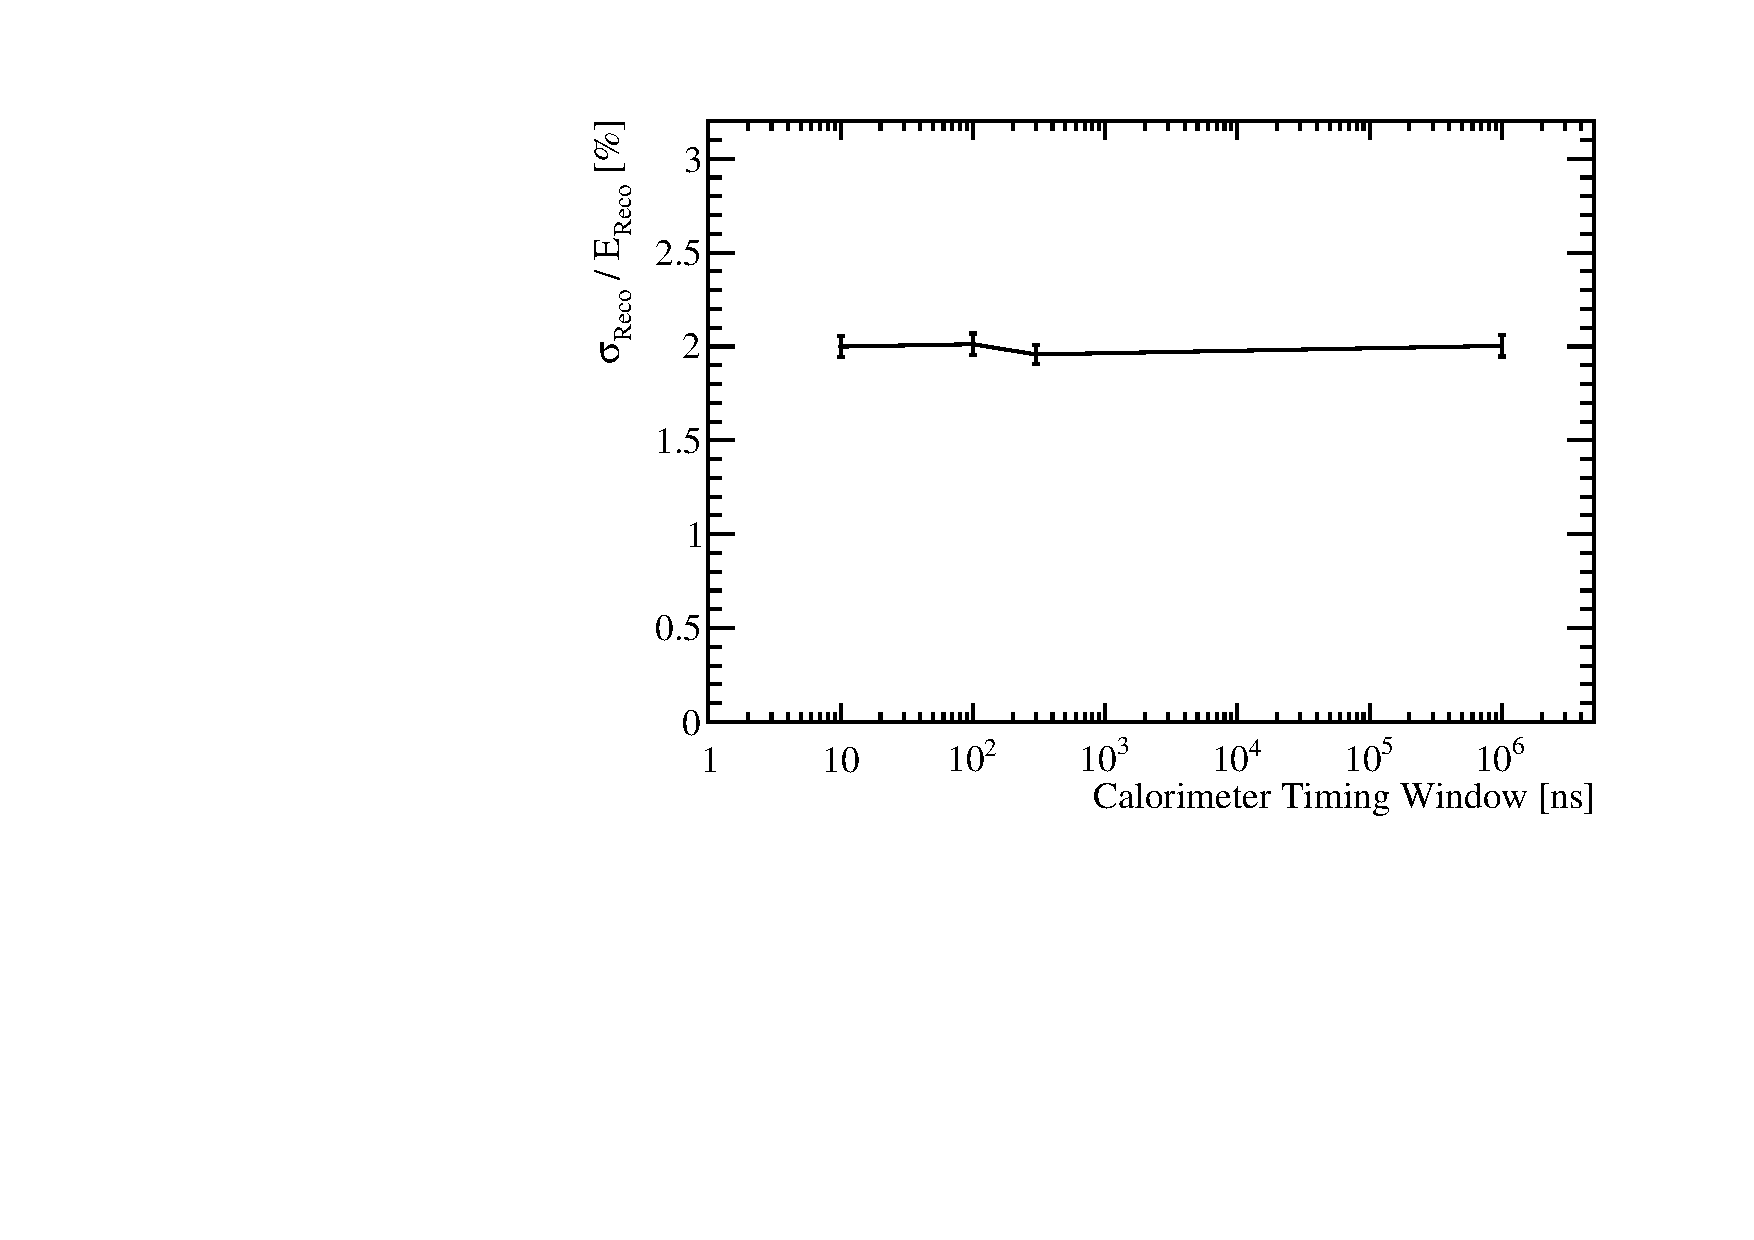
\includegraphics[width=0.5\textwidth]{EnergyEstimators/Plots/TimingCuts/ER_vs_PhotonTiming_100GeVPhoton.pdf}}
\subfloat[]{\label{fig:ertimingcutskaons}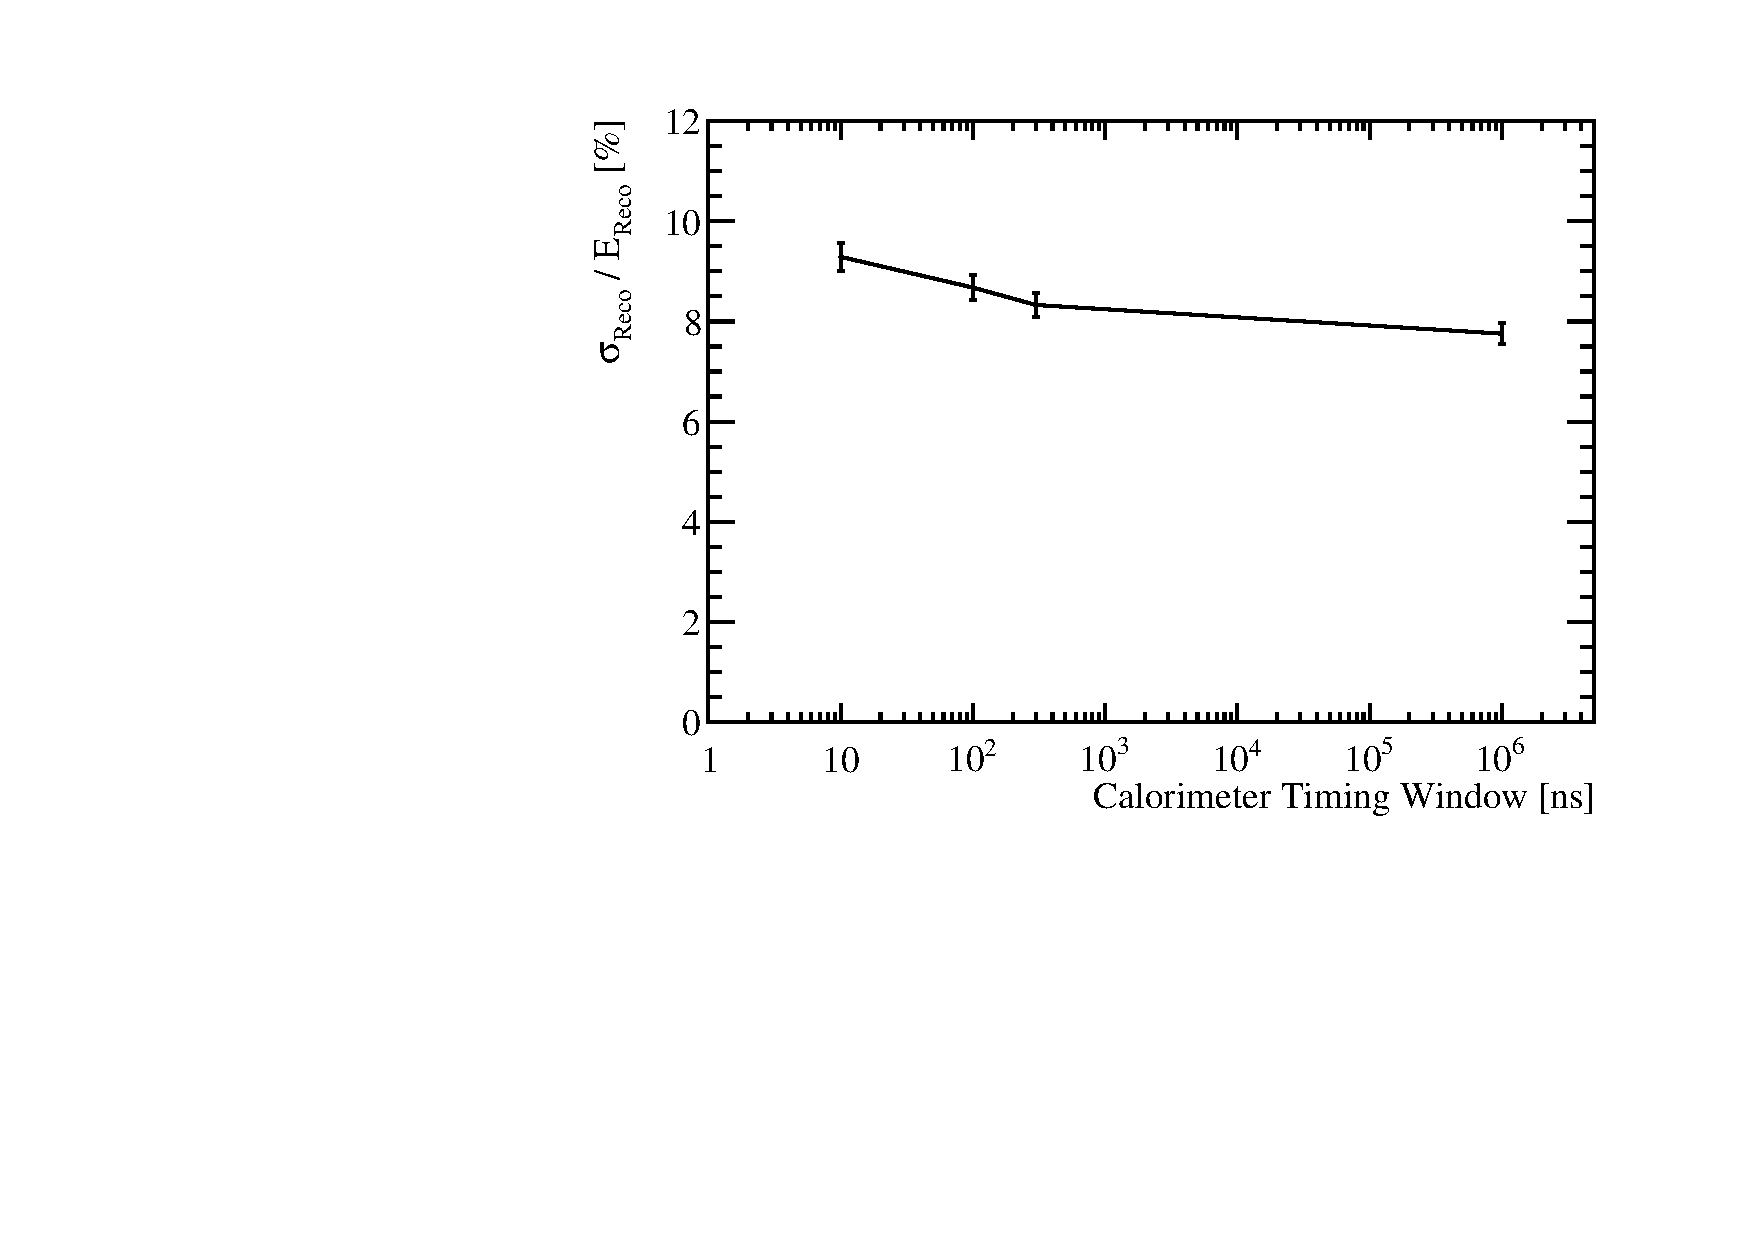
\includegraphics[width=0.5\textwidth]{EnergyEstimators/Plots/TimingCuts/ER_vs_Kaon0LTiming_50GeVKaon0L.pdf}}
\caption[The energy resolution as a function of calorimeter timing window for \protect\subref{fig:ertimingcutsphotons} 100~GeV $\gamma$ events and \protect\subref{fig:ertimingcutskaons} 50~GeV $K^{0}_{L}$ events using the nominal ILD detector model.]{The energy resolution as a function of calorimeter timing window for \protect\subref{fig:ertimingcutsphotons} 100~GeV $\gamma$ events and \protect\subref{fig:ertimingcutskaons} 50~GeV $K^{0}_{L}$ events using the nominal ILD detector model.}
\label{fig:ertimingcuts}
\end{figure}

\begin{figure}[h!]
\centering
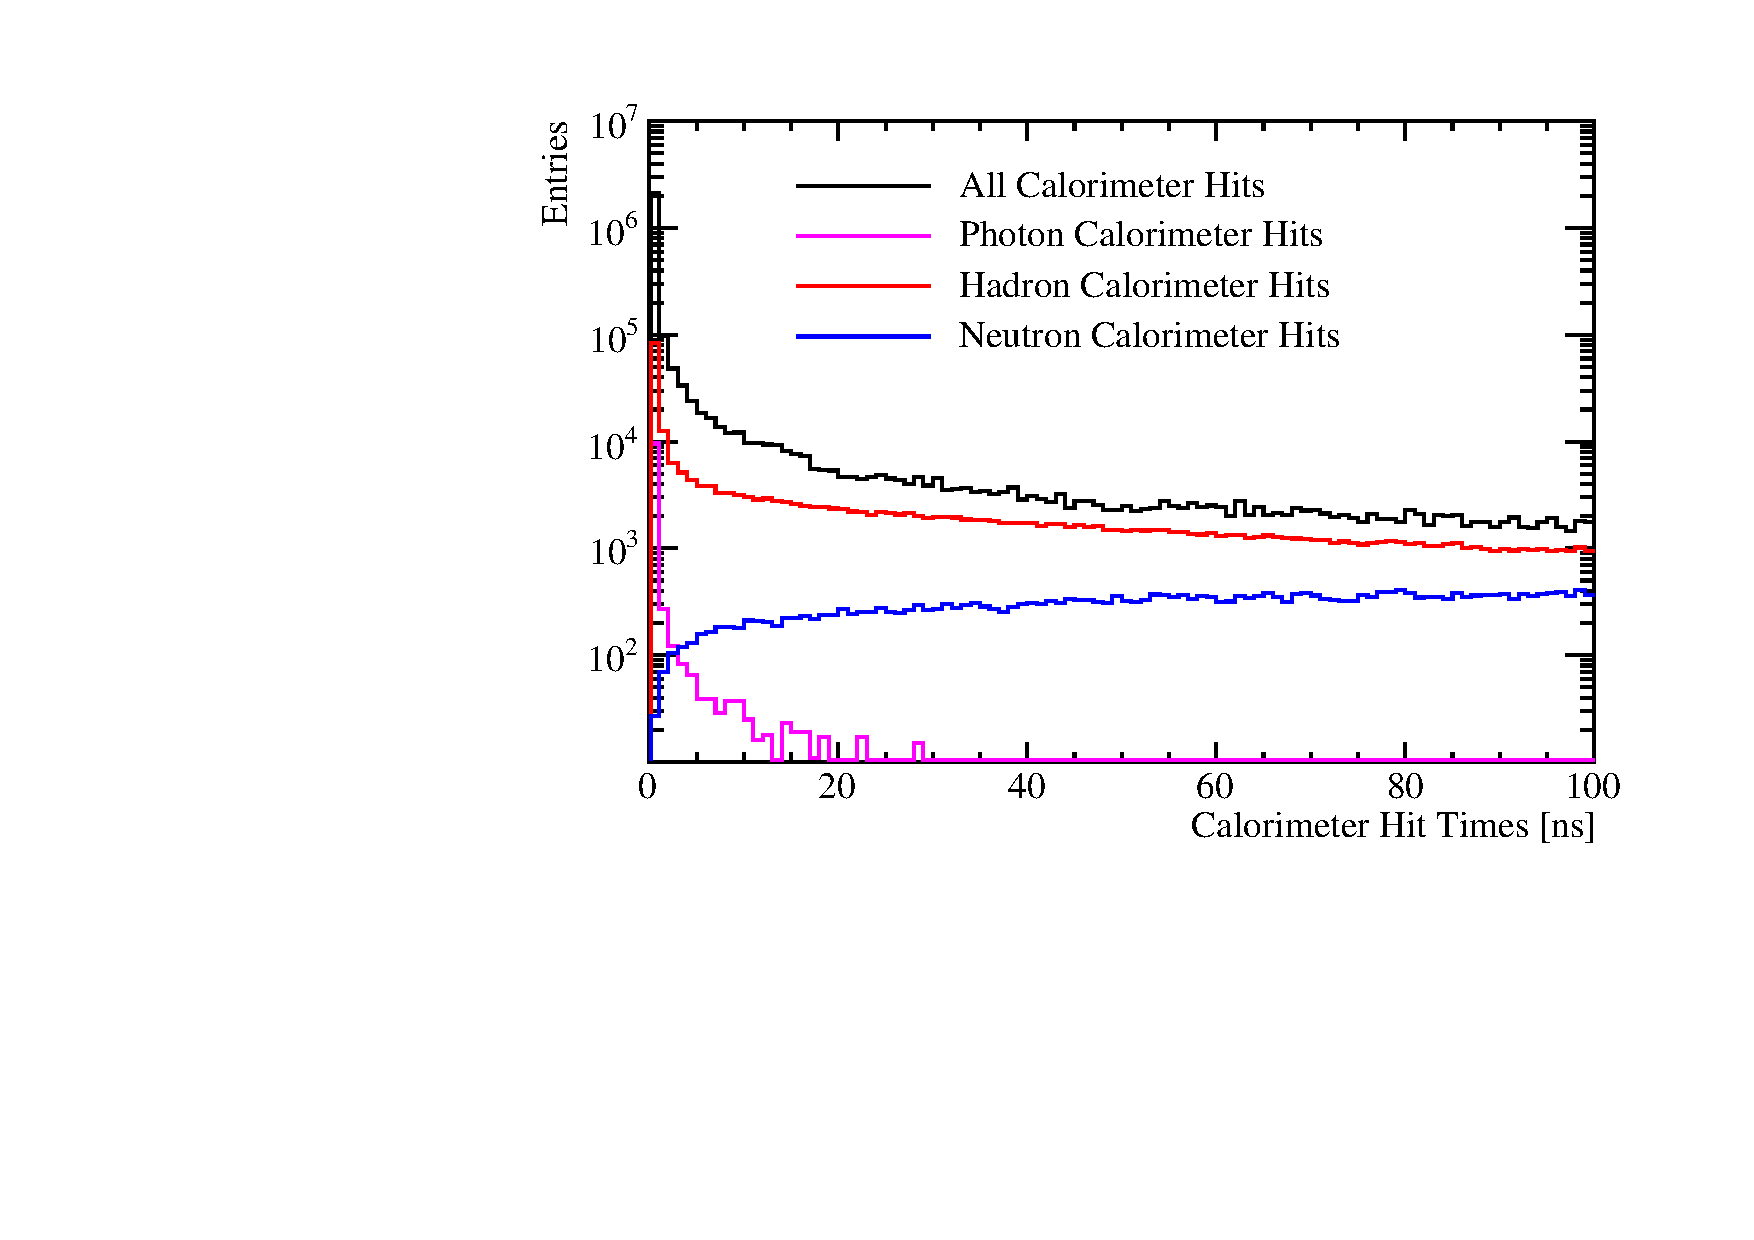
\includegraphics[width=0.5\textwidth]{OptimisationStudies/Plots/Description/CalorimeterHitTimes_91GeV_Z_uds_Steel.pdf}
\caption[The distribution of the time of the calorimeter hits, corrected for time of flight to the impact point, for 91~GeV Z$\rightarrow$uds di-jet events.]{The distribution of the time of the calorimeter hits, corrected for time of flight to the impact point, for 91~GeV Z$\rightarrow$uds di-jet events.}
\label{fig:calohittiming}
\end{figure} 

%========================================================================================

\subsubsection{Results: Jet Energy Resolution}
The jet energy resolution as a function of the jet energy for selected calorimeter time windows is shown in figure \ref{fig:jertimingcuts}.  As expected, the jet energy resolution will also be affected by the reduced neutral hadron energy resolution when the calorimeter timing window is reduced.  The sole exception to this is the 250~GeV jets for the 100~ns time window whereby the jet energy resolution is slightly better than when using the 300~ns and semi-infinite time windows.  As the magnitude of the changes to the jet energy resolution when varying the time window size are small in comparison to the absolute resolutions, this exception will most likely be due to a fluctuation in either the event sample used or in the application of the calibration procedure.  

\begin{figure}[h!]
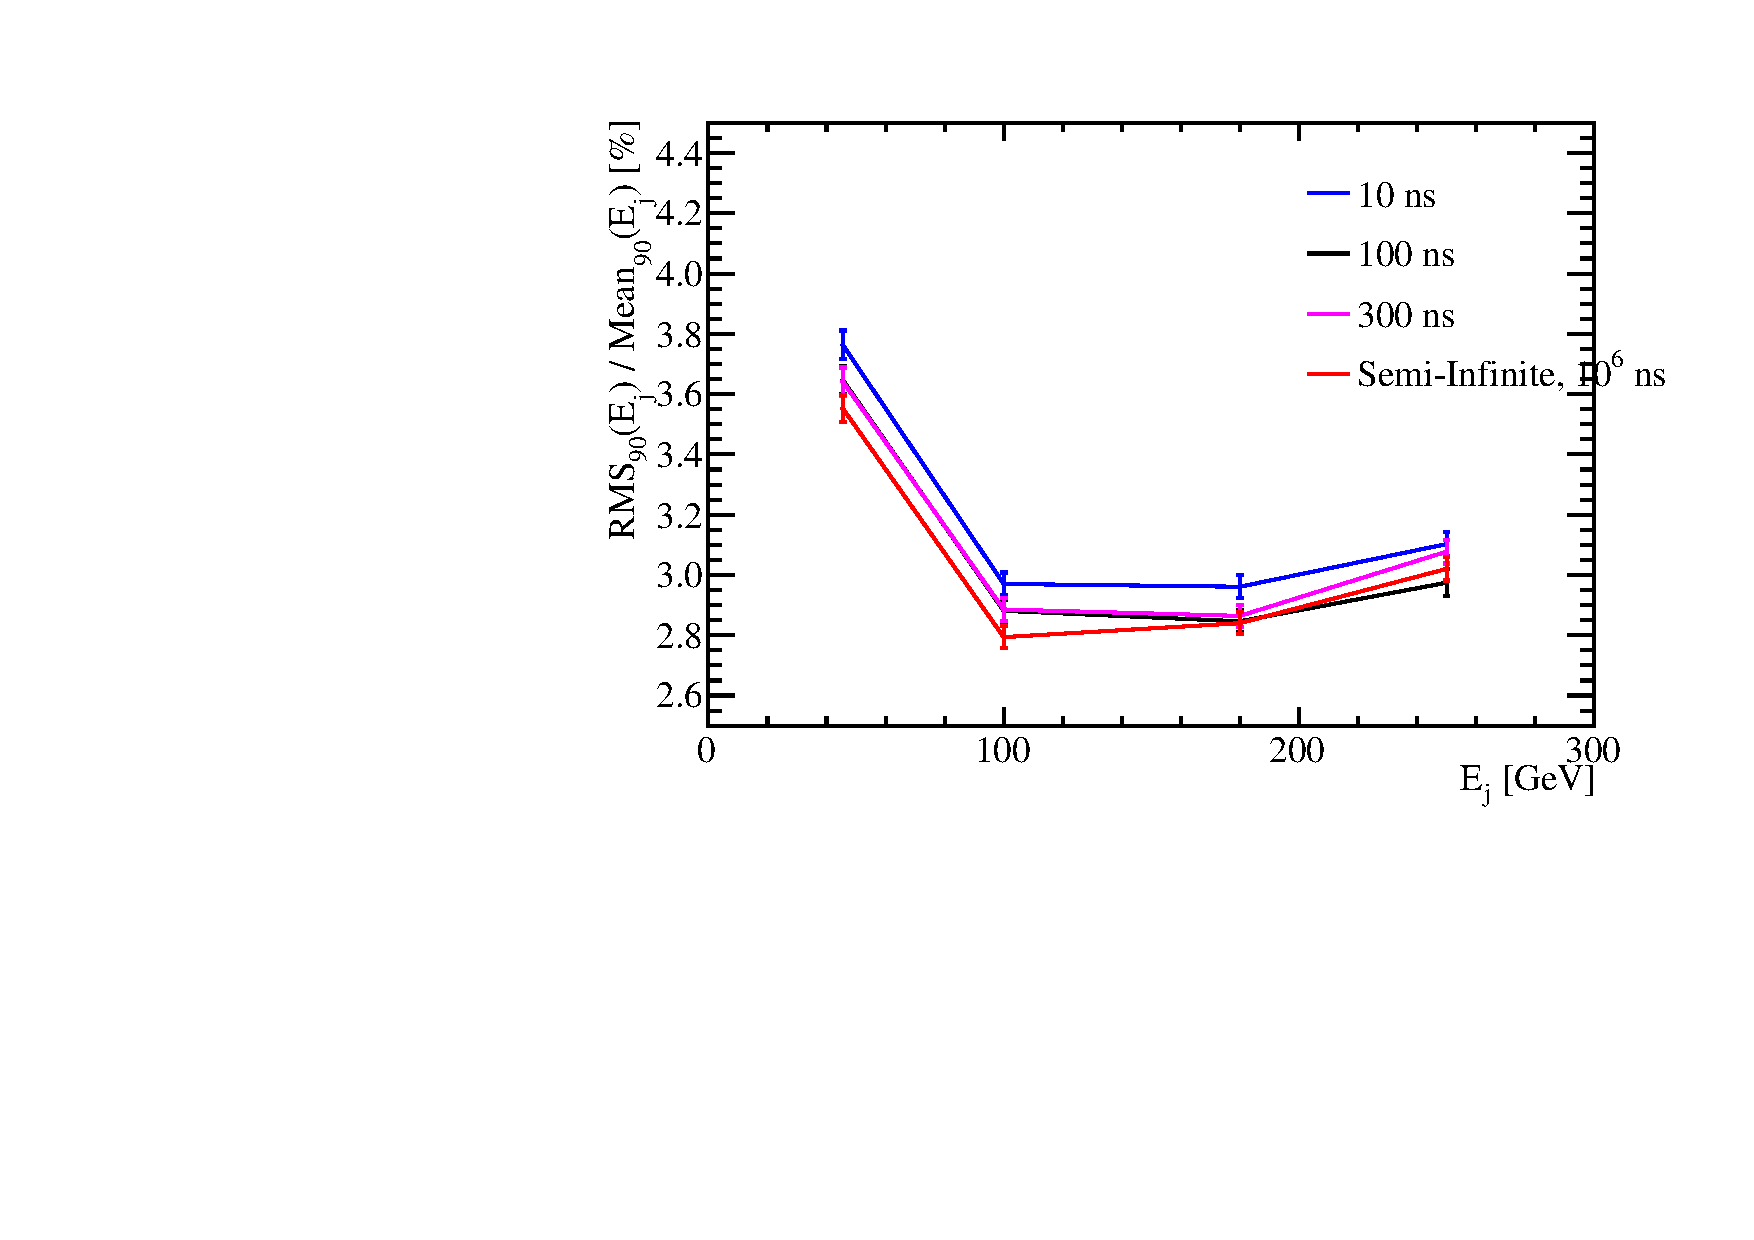
\includegraphics[width=0.5\textwidth]{EnergyEstimators/Plots/TimingCuts/JER_vs_JetEnergy_TimingCutStudies.pdf}
\caption[The jet energy resolution as a function of jet energy for various calorimeter timing cuts.  The results shown use the nominal ILD detector model.]{The jet energy resolution as a function of jet energy for various calorimeter timing cuts.  The nominal ILD detector model was used for this study.}
\label{fig:jertimingcuts}
\end{figure}

The time window applied to the calorimeter hits affects both the neutral hadron and jet energy resolutions with a larger timing window leading to better resolutions.  It can be seen that applying an aggressive choice of time window, such as 10~ns, the jet energy resolution is degraded as many of the hadronic showers being sampled do not have time to fully develop.  However, even using a 10~ns timing cut the jet energy resolutions are still sufficiently low to give excellent detector performance.  Both the single particle and jet energy resolutions indicate that the majority of hadronic showers will have fully developed within 100~ns and that there are little gains to be made by extending the size of this window.  

For results presented in this chapter and the optimisation studies found in chapter \ref{chap:detopt} a 100~ns timing window was applied across all models considered.  As the choice of timing window has yet to be finalised for the linear collider this value was chosen as it represents something that could be achieved using the readout technology options presently available \cite{Adloff:2014rya}.  Furthermore, it adds additional realism to the detector simulation in comparison to omitting the effect of the calorimeter time window.  The categorisation of changes to the detector performance when varying the calorimeter timing window presented here can be used to discern the impact of changing the timing window used for the optimisation studies at a later date if so desired.  

%========================================================================================
%========================================================================================
